% =====================================================================
% Chapter 5: Results and Analysis
% =====================================================================
\chapter{Results and Analysis}
\label{ch:results}

\section{Overview}

This chapter presents the quantitative and qualitative results from
both pipelines. Section~\ref{sec:results-legibility} covers legibility
classifier training results in detail.
Section~\ref{sec:results-image-demo} demonstrates the image pipeline
on a sample image. Sections~\ref{sec:results-freq}--\ref{sec:results-confidence}
present player-level accuracy, confusion matrix, and OCR confidence
analysis. Section~\ref{sec:results-video} presents the video pipeline
tracking and OCR results. Section~\ref{sec:lit-comparison} places
the results in context by comparison with prior work.

\section{Legibility Classifier Training Results}
\label{sec:results-legibility}

The ResNet-18 legibility classifier was trained for 20 epochs on
weakly-labeled crops derived from the OCR manifest.
Figure~\ref{fig:legibility-curves} provides a combined overview of
the training history, showing both loss and accuracy curves across all
epochs in a single view. This combined plot makes it straightforward
to correlate the point at which validation loss reaches its minimum
(epoch 5) with the peak in validation accuracy (epoch 6), supporting
the checkpointing decision described in
Section~\ref{sec:legibility-training}.

\begin{figure}[H]
    \centering
    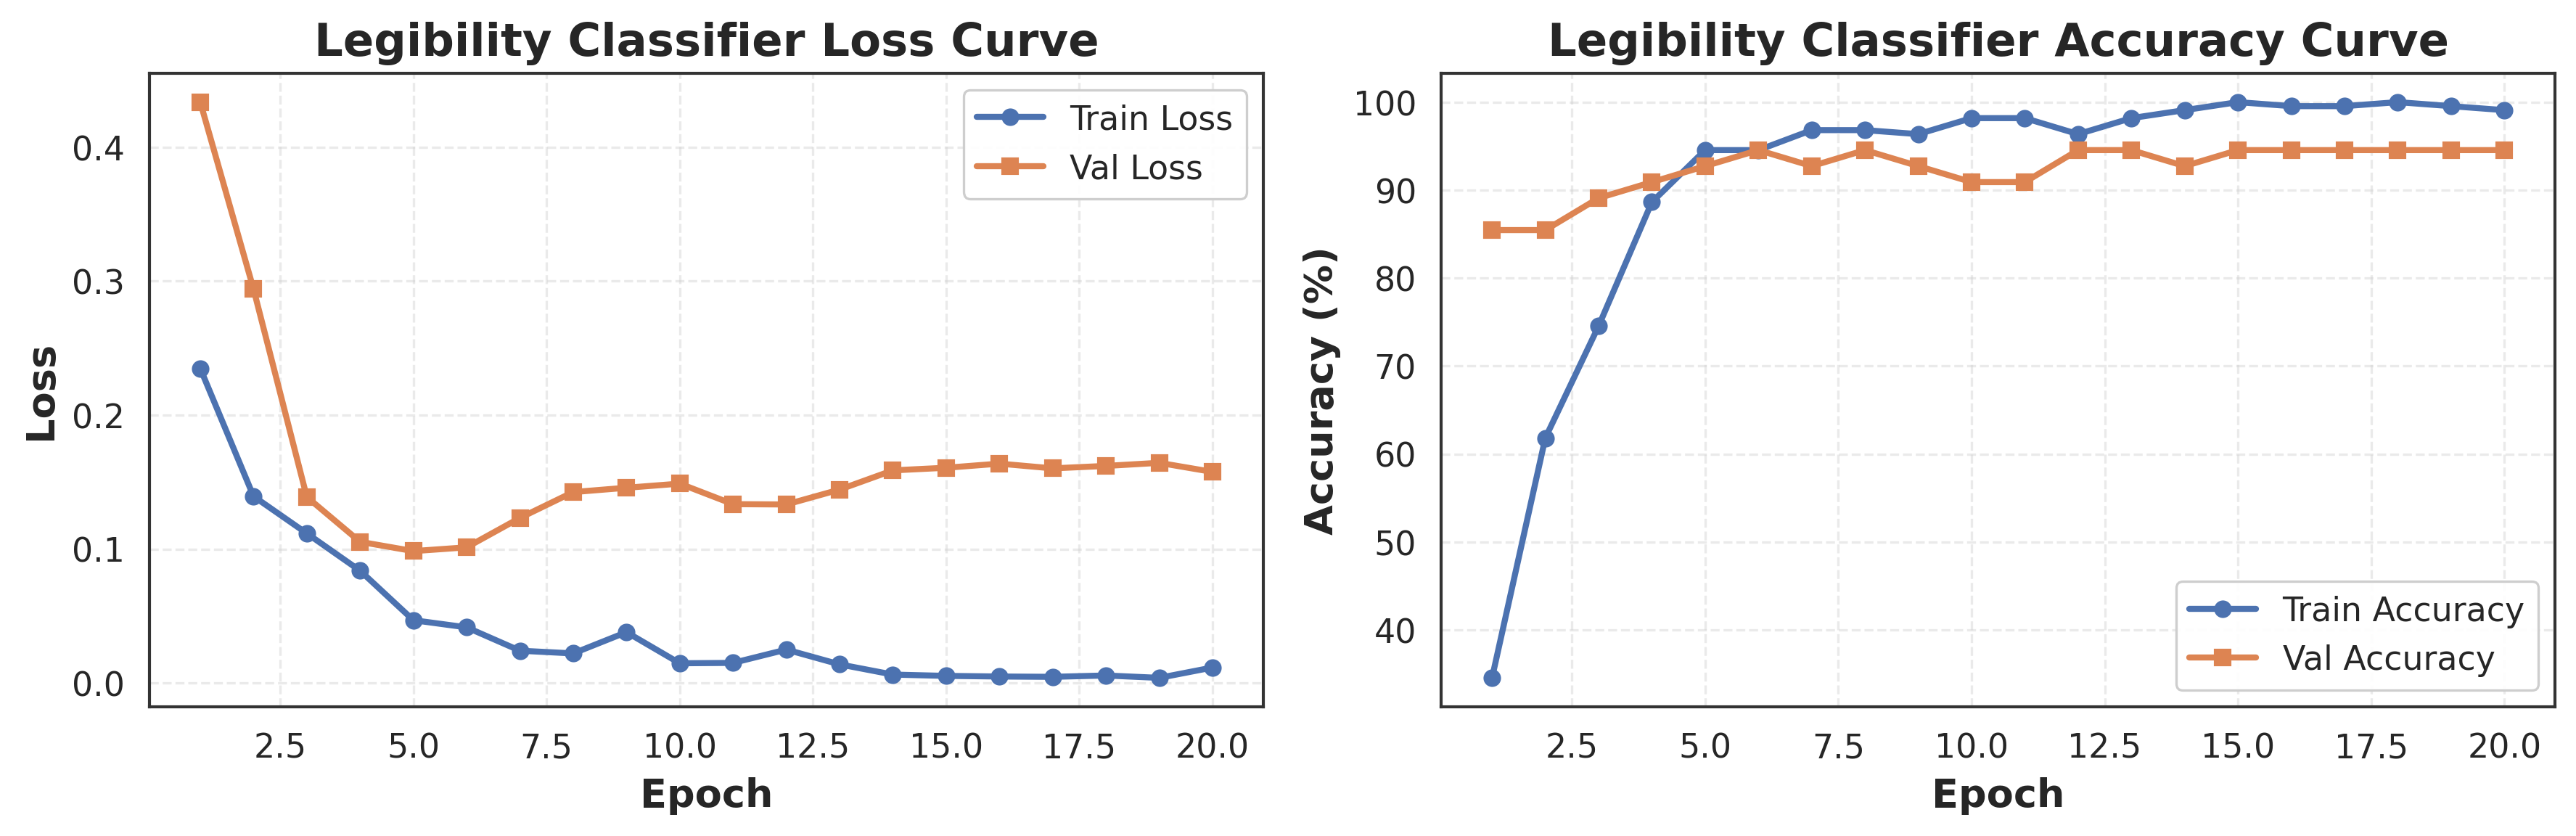
\includegraphics[width=\textwidth]{figures/legibility_curves.jpg}
    \caption{Combined training history of the ResNet-18 legibility
    classifier: training and validation loss (left) and training and
    validation accuracy (right) across 20 epochs. Training loss
    converges to near zero, while validation accuracy peaks at
    \textbf{94.55\%} at epoch~6. The gradual rise in validation loss
    after epoch~5 indicates the onset of mild overfitting, confirming
    that the checkpoint saved around epoch~5--6 is the optimal one.}
    \label{fig:legibility-curves}
\end{figure}

Figure~\ref{fig:legibility-curves} above already shows both curves
in detail; the combined view makes it easy to see that the minimum
validation loss (epoch~5) closely precedes the peak validation accuracy
(epoch~6), confirming the choice of this region as the best checkpoint.

Figures~\ref{fig:legibility-pr} and~\ref{fig:legibility-roc} present
the precision-recall and ROC curves computed on the validation set,
evaluating the classifier across all possible decision thresholds rather
than at a single operating point.

\begin{figure}[H]
    \centering
    \begin{subfigure}[t]{0.47\textwidth}
        \centering
        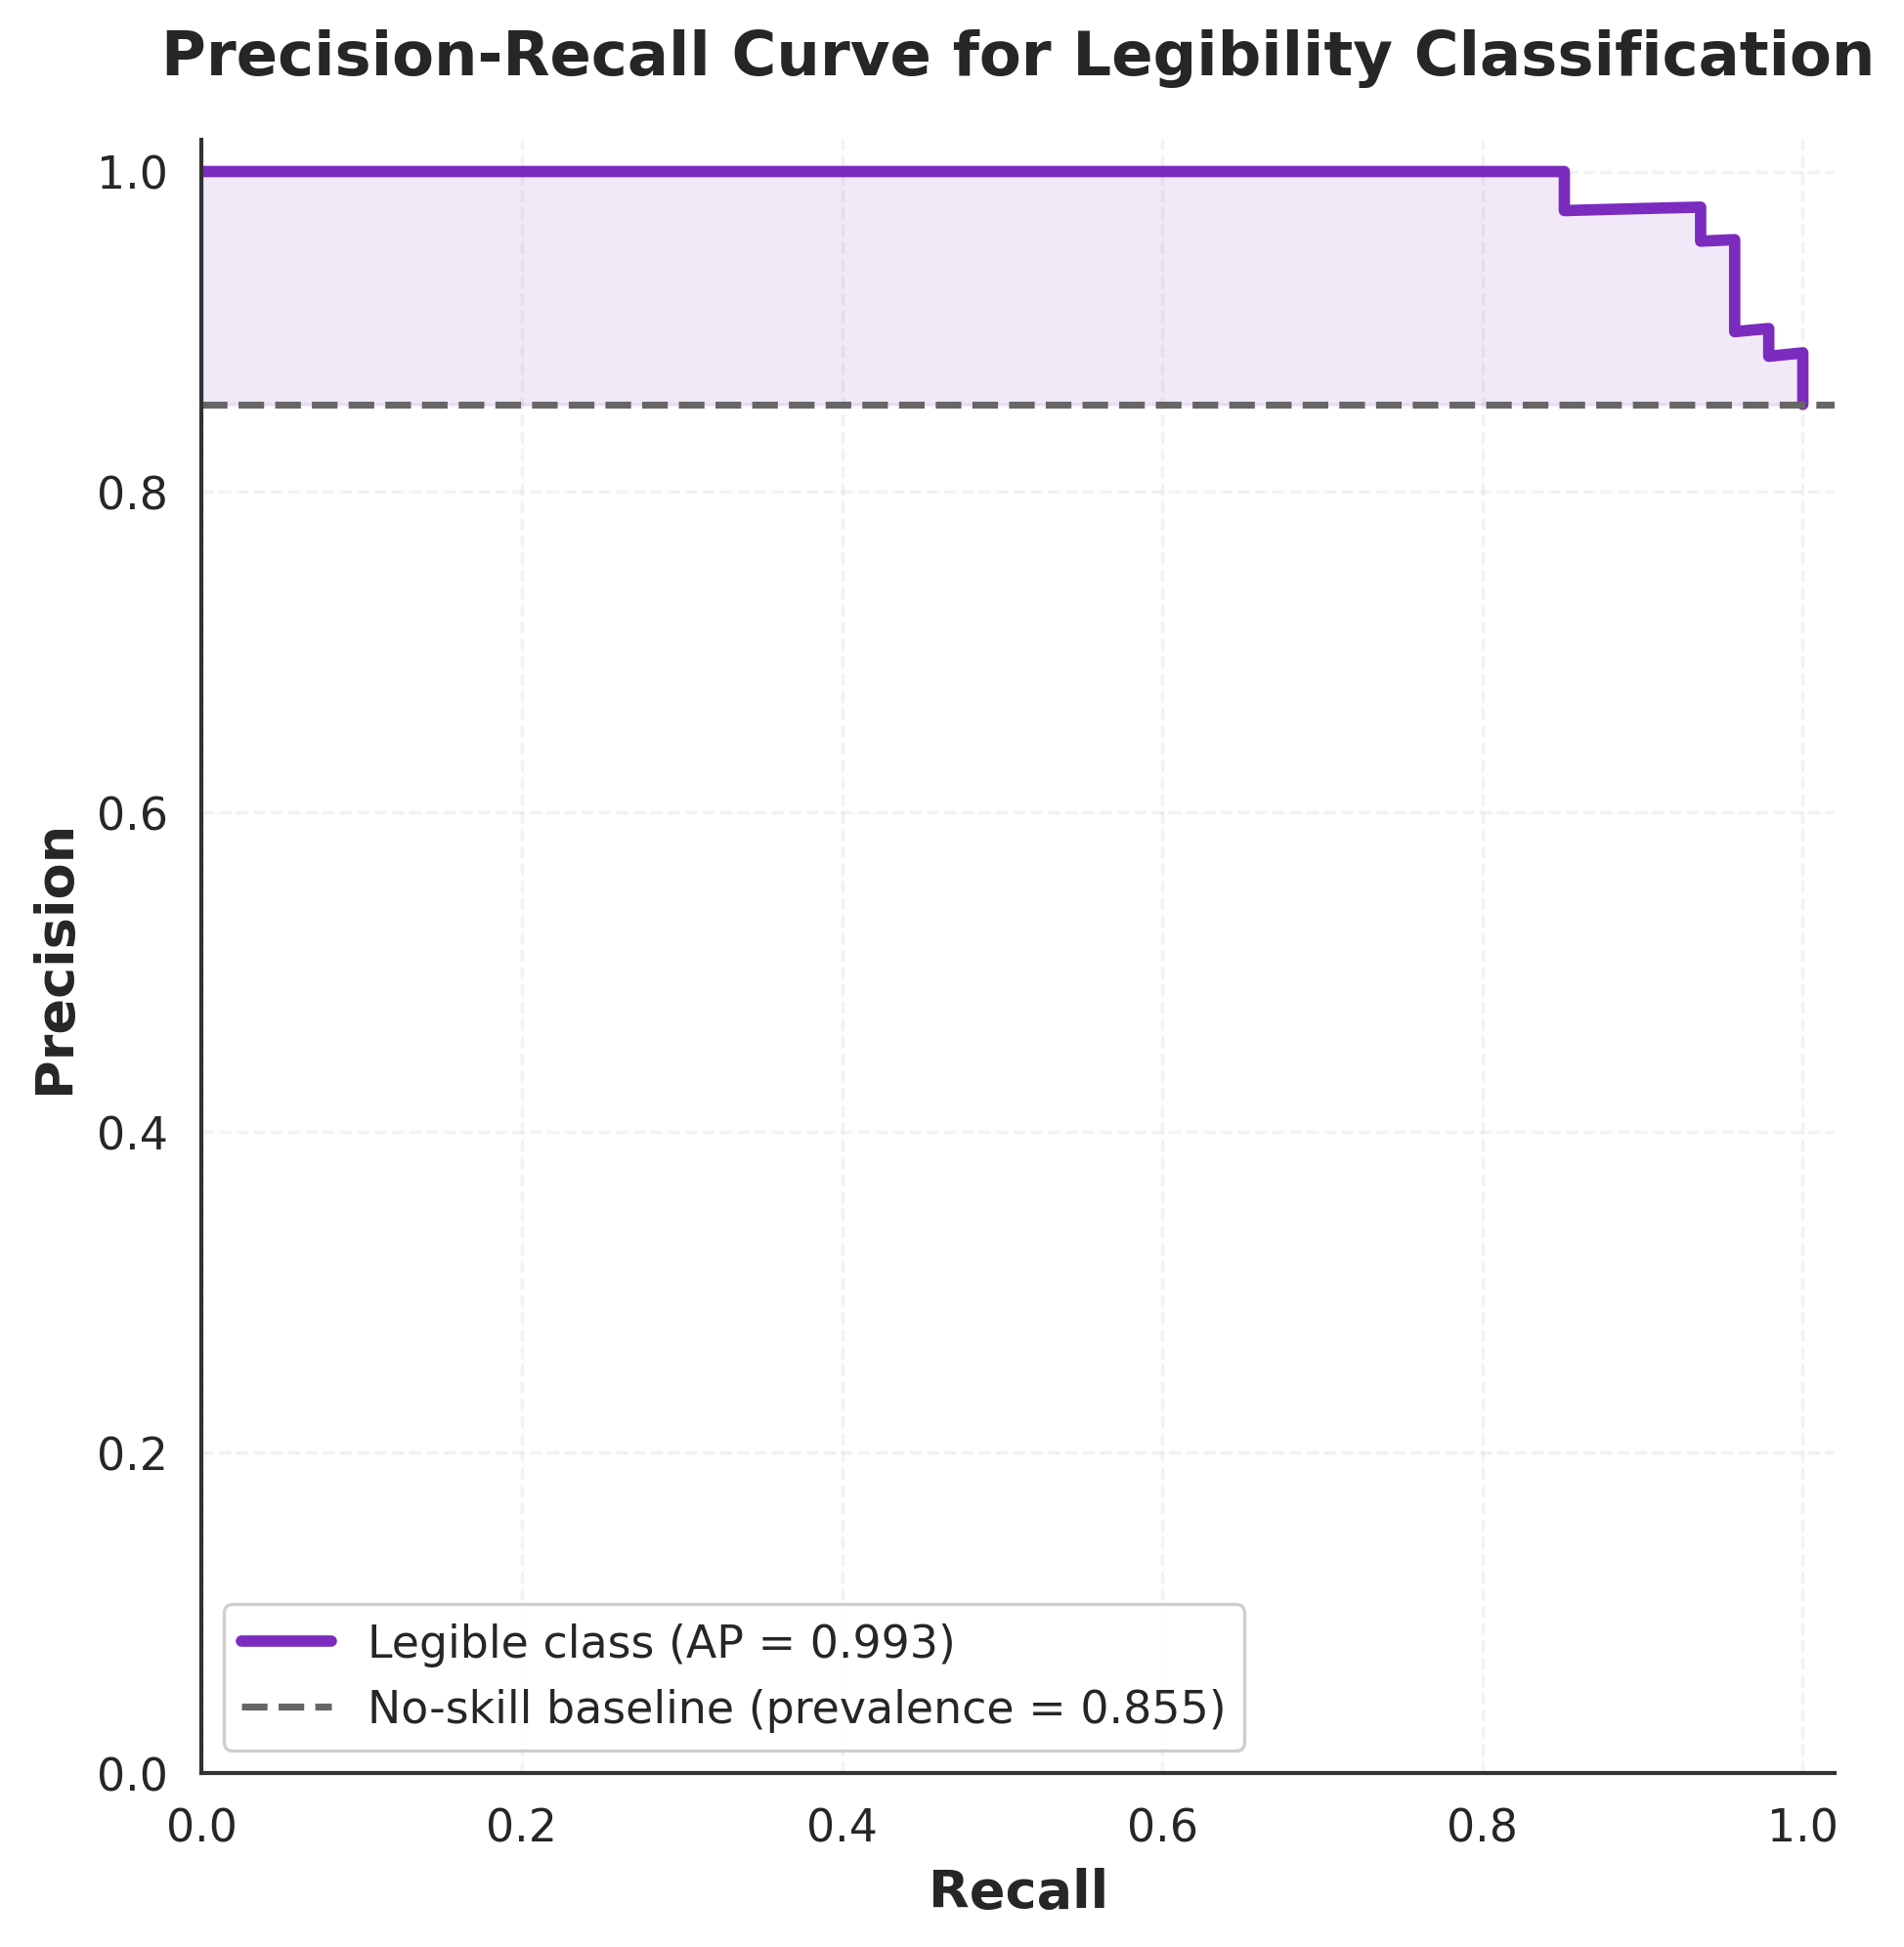
\includegraphics[width=\textwidth]{figures/fig_legibility_pr.jpg}
        \caption{Precision-Recall curve (AP = 0.993).}
        \label{fig:legibility-pr}
    \end{subfigure}
    \hfill
    \begin{subfigure}[t]{0.47\textwidth}
        \centering
        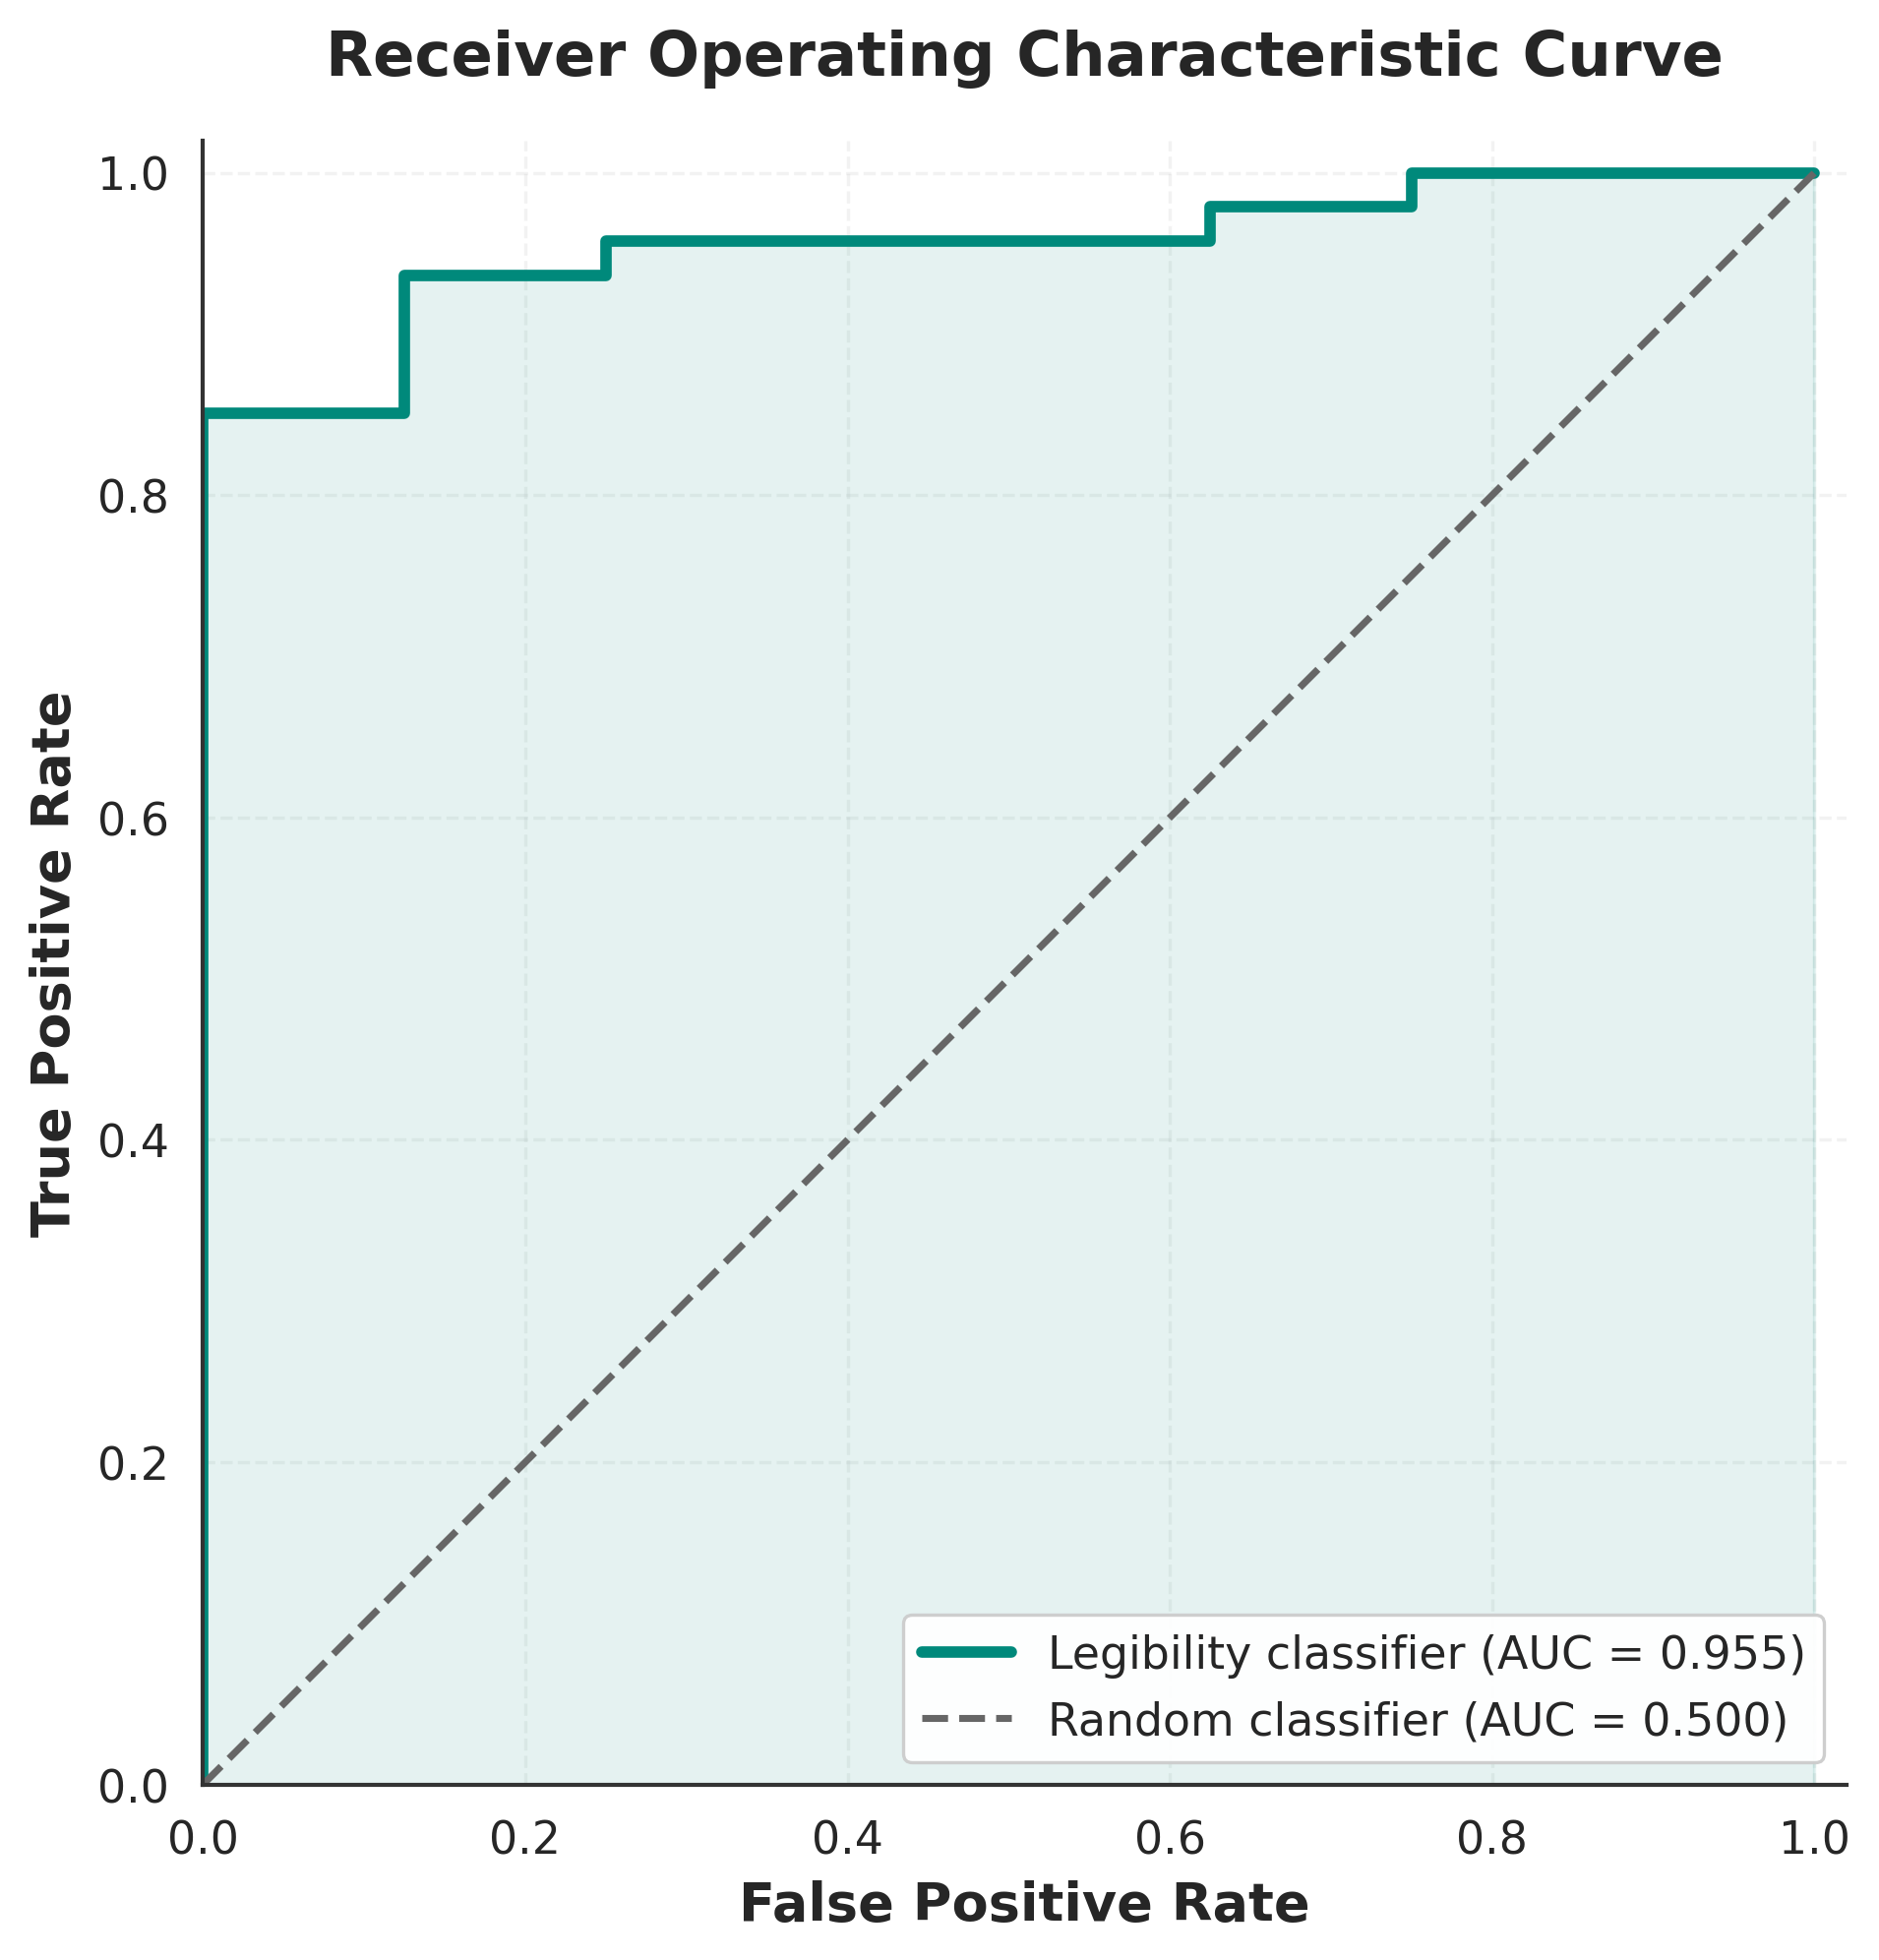
\includegraphics[width=\textwidth]{figures/fig_legibility_roc.jpg}
        \caption{ROC curve (AUC = 0.955).}
        \label{fig:legibility-roc}
    \end{subfigure}
    \caption{Legibility classifier PR and ROC curves on the validation
    set. The near-perfect average precision (0.993) confirms that
    the classifier maintains high precision even at high recall. The
    AUC of 0.955 indicates strong discriminative ability between
    legible and illegible crops across all thresholds, with the
    optimal threshold lying near the top-left corner of the ROC plot.}
    \label{fig:legibility-curves-combined}
\end{figure}

Figure~\ref{fig:legibility-per-class} shows per-class accuracy on the
47 validation samples labeled \textit{Legible} and the 8 labeled
\textit{Illegible}.

\begin{figure}[H]
    \centering
    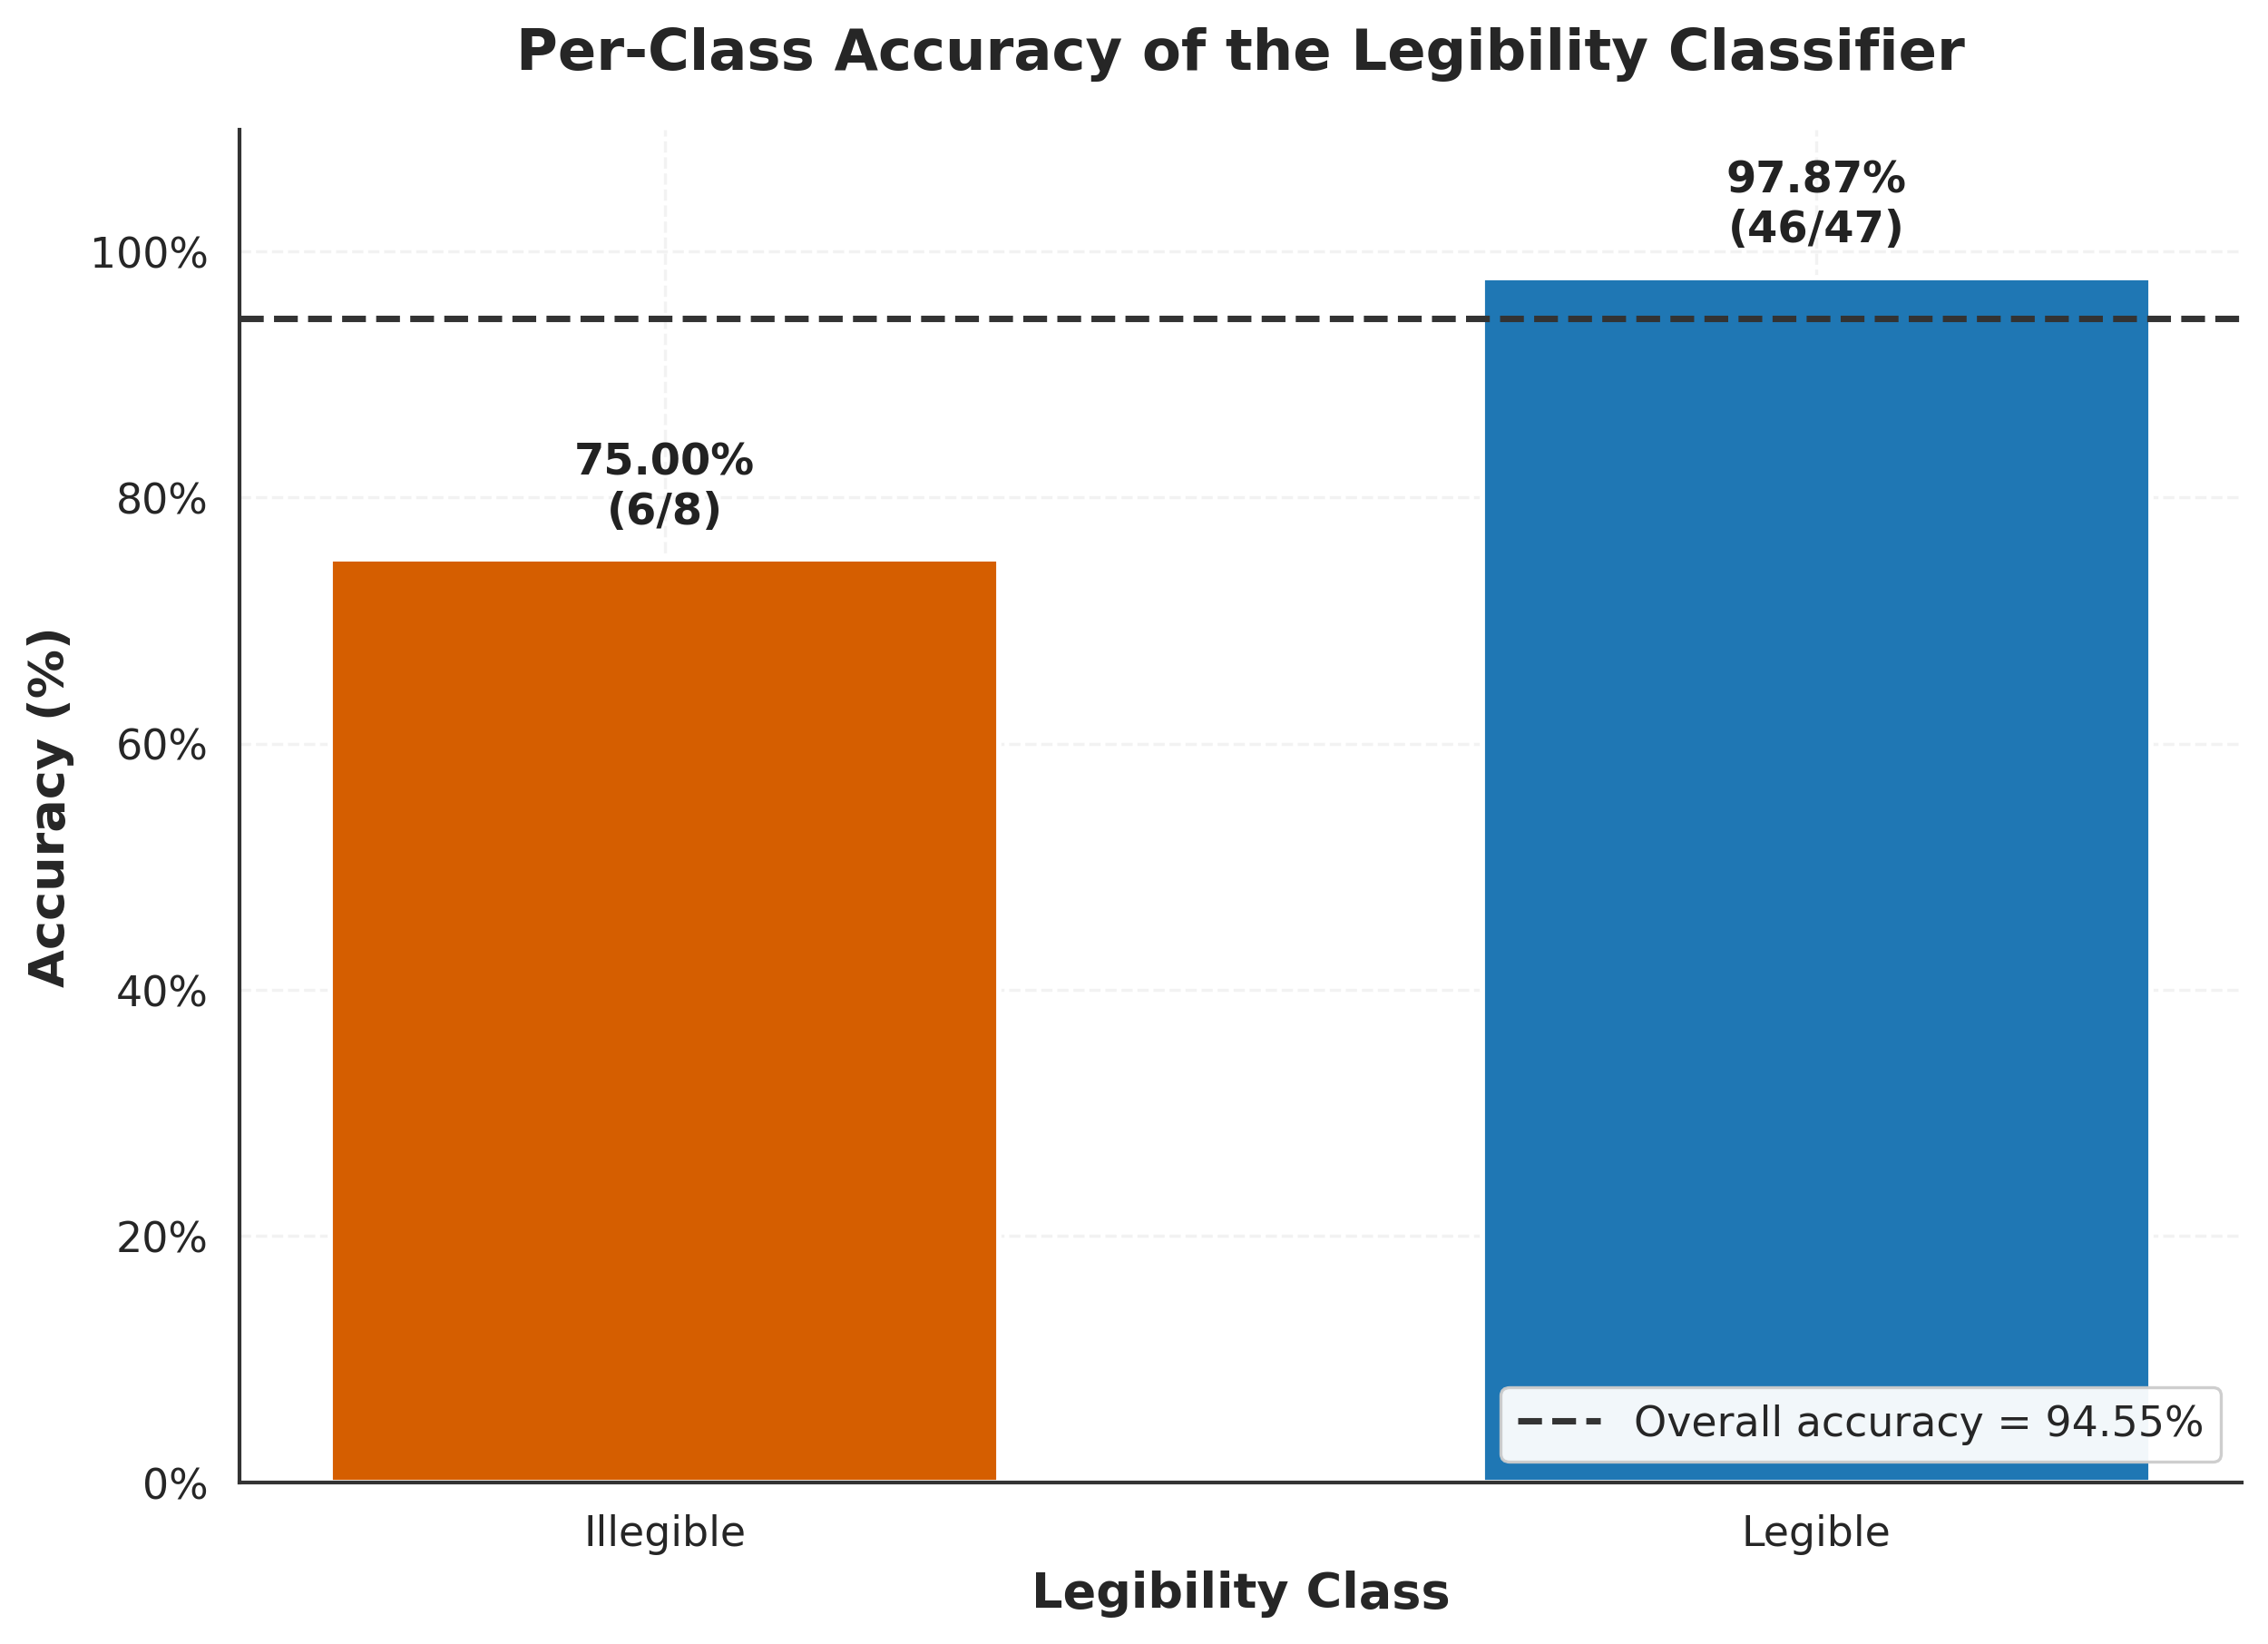
\includegraphics[width=0.75\textwidth]{figures/fig_legibility_per_class.jpg}
    \caption{Per-class validation accuracy: \textbf{97.87\%} for
    \textit{Legible} (47 samples) and \textbf{75.00\%} for
    \textit{Illegible} (8 samples). The lower accuracy on the
    \textit{Illegible} class reflects both its smaller sample count
    and the inherent ambiguity of crops that are borderline legible ---
    cases where human labelers and the OCR confidence threshold would
    also disagree; each of the two misclassified illegible crops shifts
    this class accuracy by 12.5 percentage points, which is why it is
    considerably more volatile across training runs than the
    \textit{Legible} class accuracy.}
    \label{fig:legibility-per-class}
\end{figure}

Table~\ref{tab:legibility-summary} summarizes all key legibility
classifier metrics.

\begin{table}[H]
    \centering
    \caption{Legibility classifier summary metrics on the validation set.}
    \label{tab:legibility-summary}
    \begin{tabular}{@{}lr@{}}
        \toprule
        \textbf{Metric} & \textbf{Value} \\
        \midrule
        Validation samples & 55 \\
        Overall validation accuracy & 94.55\% \\
        Best epoch (by val accuracy) & Epoch 6 \\
        Minimum validation loss & 0.0984 (epoch 5) \\
        Average precision (PR curve) & 0.993 \\
        ROC-AUC & 0.955 \\
        \textit{Legible} class accuracy & 97.87\% (47 samples) \\
        \textit{Illegible} class accuracy & 75.00\% (8 samples) \\
        \bottomrule
    \end{tabular}
\end{table}

\section{Image Pipeline: End-to-End Demonstration}
\label{sec:results-image-demo}

Figure~\ref{fig:demo-recap} illustrates the complete image pipeline
for a single player sample, showing every intermediate stage from raw
input to enhanced OCR variants. The example demonstrates the combined
effect of pose-driven torso localization (narrowing the search region)
and the enhancement stages (improving digit contrast and sharpness)
before the multi-variant OCR engine reads the jersey number.

\begin{figure}[H]
    \centering
    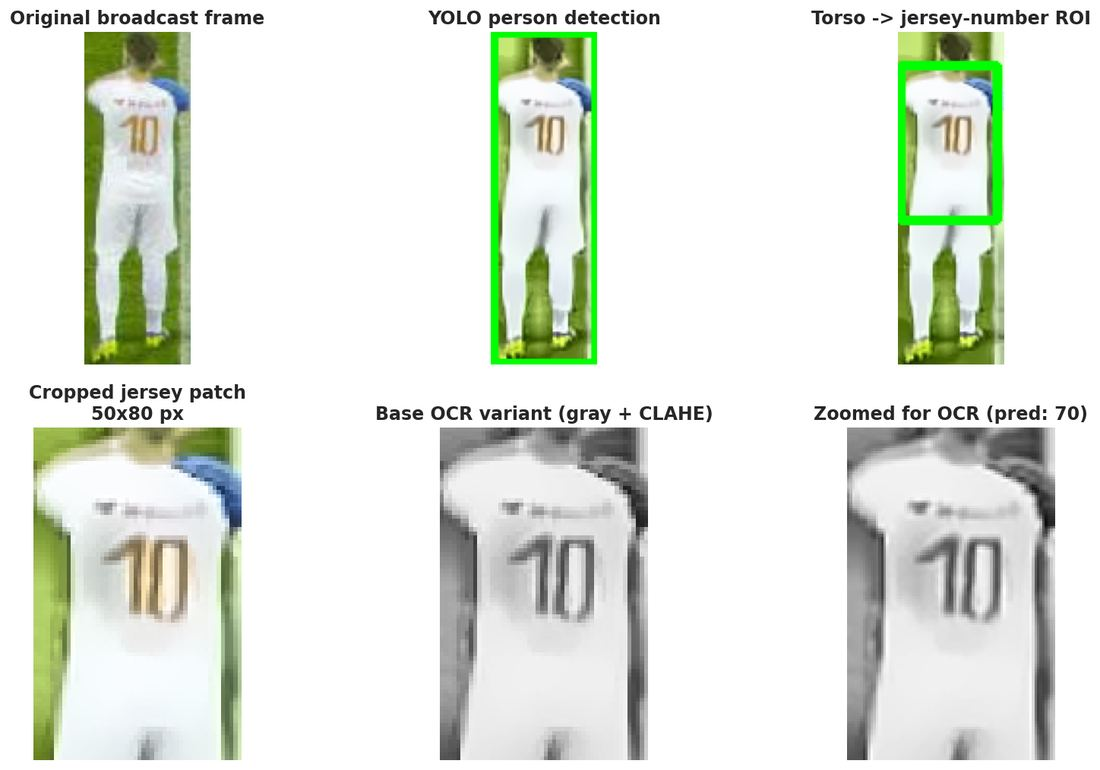
\includegraphics[width=\textwidth]{figures/fig_image_pipeline_demo.jpg}
    \caption{Full image pipeline demonstration on one SoccerNet sample.
    The leftmost column shows the original image and the YOLOv8x
    detection box; the middle column shows the torso localization and
    jersey-number ROI derived from YOLOv8x-Pose keypoints; the
    rightmost column shows the raw crop at native resolution and the
    CLAHE-enhanced, upscaled variant fed to EasyOCR. The multi-variant
    OCR engine correctly identifies the jersey number from the enhanced
    patch.}
    \label{fig:demo-recap}
\end{figure}

\section{Jersey-Number Frequency Distribution}
\label{sec:results-freq}

Figure~\ref{fig:jersey-freq} shows the ground-truth jersey number
distribution across the evaluated image subset. The distribution is
highly right-skewed, with jersey number \textbf{10} appearing far more
frequently than any other number. This is consistent with the iconic
status of the No.\ 10 shirt in football, which is typically assigned to
the playmaker. The next most common numbers --- 4, 8, 24, and 30 ---
reflect the jersey allocation patterns found in the specific SoccerNet
sequences sampled. This skew is worth bearing in mind when interpreting
the confusion matrix (Section~\ref{sec:results-confusion}): high
per-number accuracy for jersey 10 carries disproportionate weight in
the overall player-level accuracy figure.

\begin{figure}[H]
    \centering
    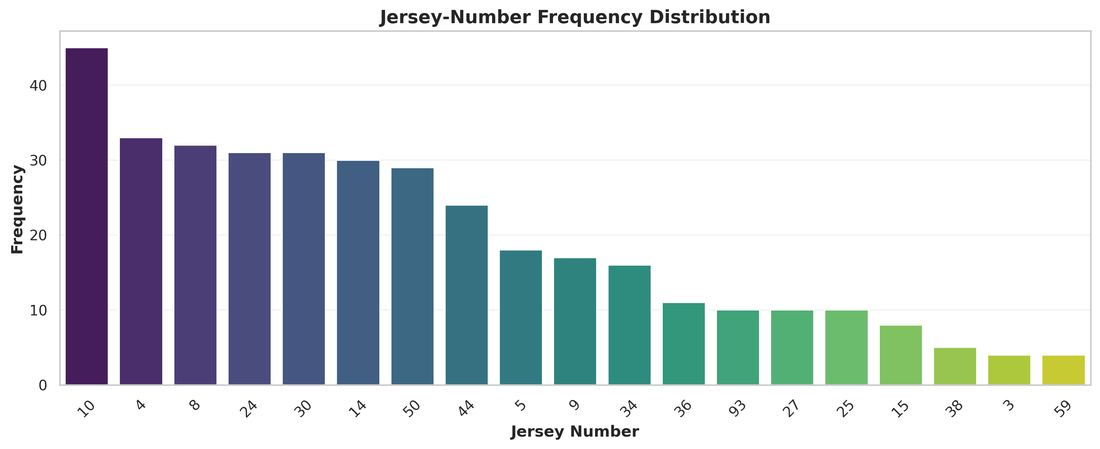
\includegraphics[width=1\textwidth]{figures/fig_jersey_freq_distribution.jpg}
    \caption{Frequency distribution of ground-truth jersey numbers in
    the evaluated dataset subset. Jersey number 10 is by far the most
    frequent (approximately 45 occurrences), followed by 4, 8, 24, and
    30. Numbers in the range 1--9 (single-digit) collectively appear
    less often than common two-digit numbers, reflecting their relative
    scarcity in the positions sampled.}
    \label{fig:jersey-freq}
\end{figure}

\section{Player-Level Prediction Examples}

Figures~\ref{fig:train-player-pred-0} and~\ref{fig:train-player-pred-1}
present detailed qualitative case studies for two representative
training-set players, and Figures~\ref{fig:test-player-pred-0}
and~\ref{fig:test-player-pred-1} present the corresponding case studies
for two representative test-set players. Each figure shows the six
individual crops contributing to that player's folder together with
the pipeline's final mode-aggregated jersey-number prediction.

\begin{figure}[H]
    \centering
    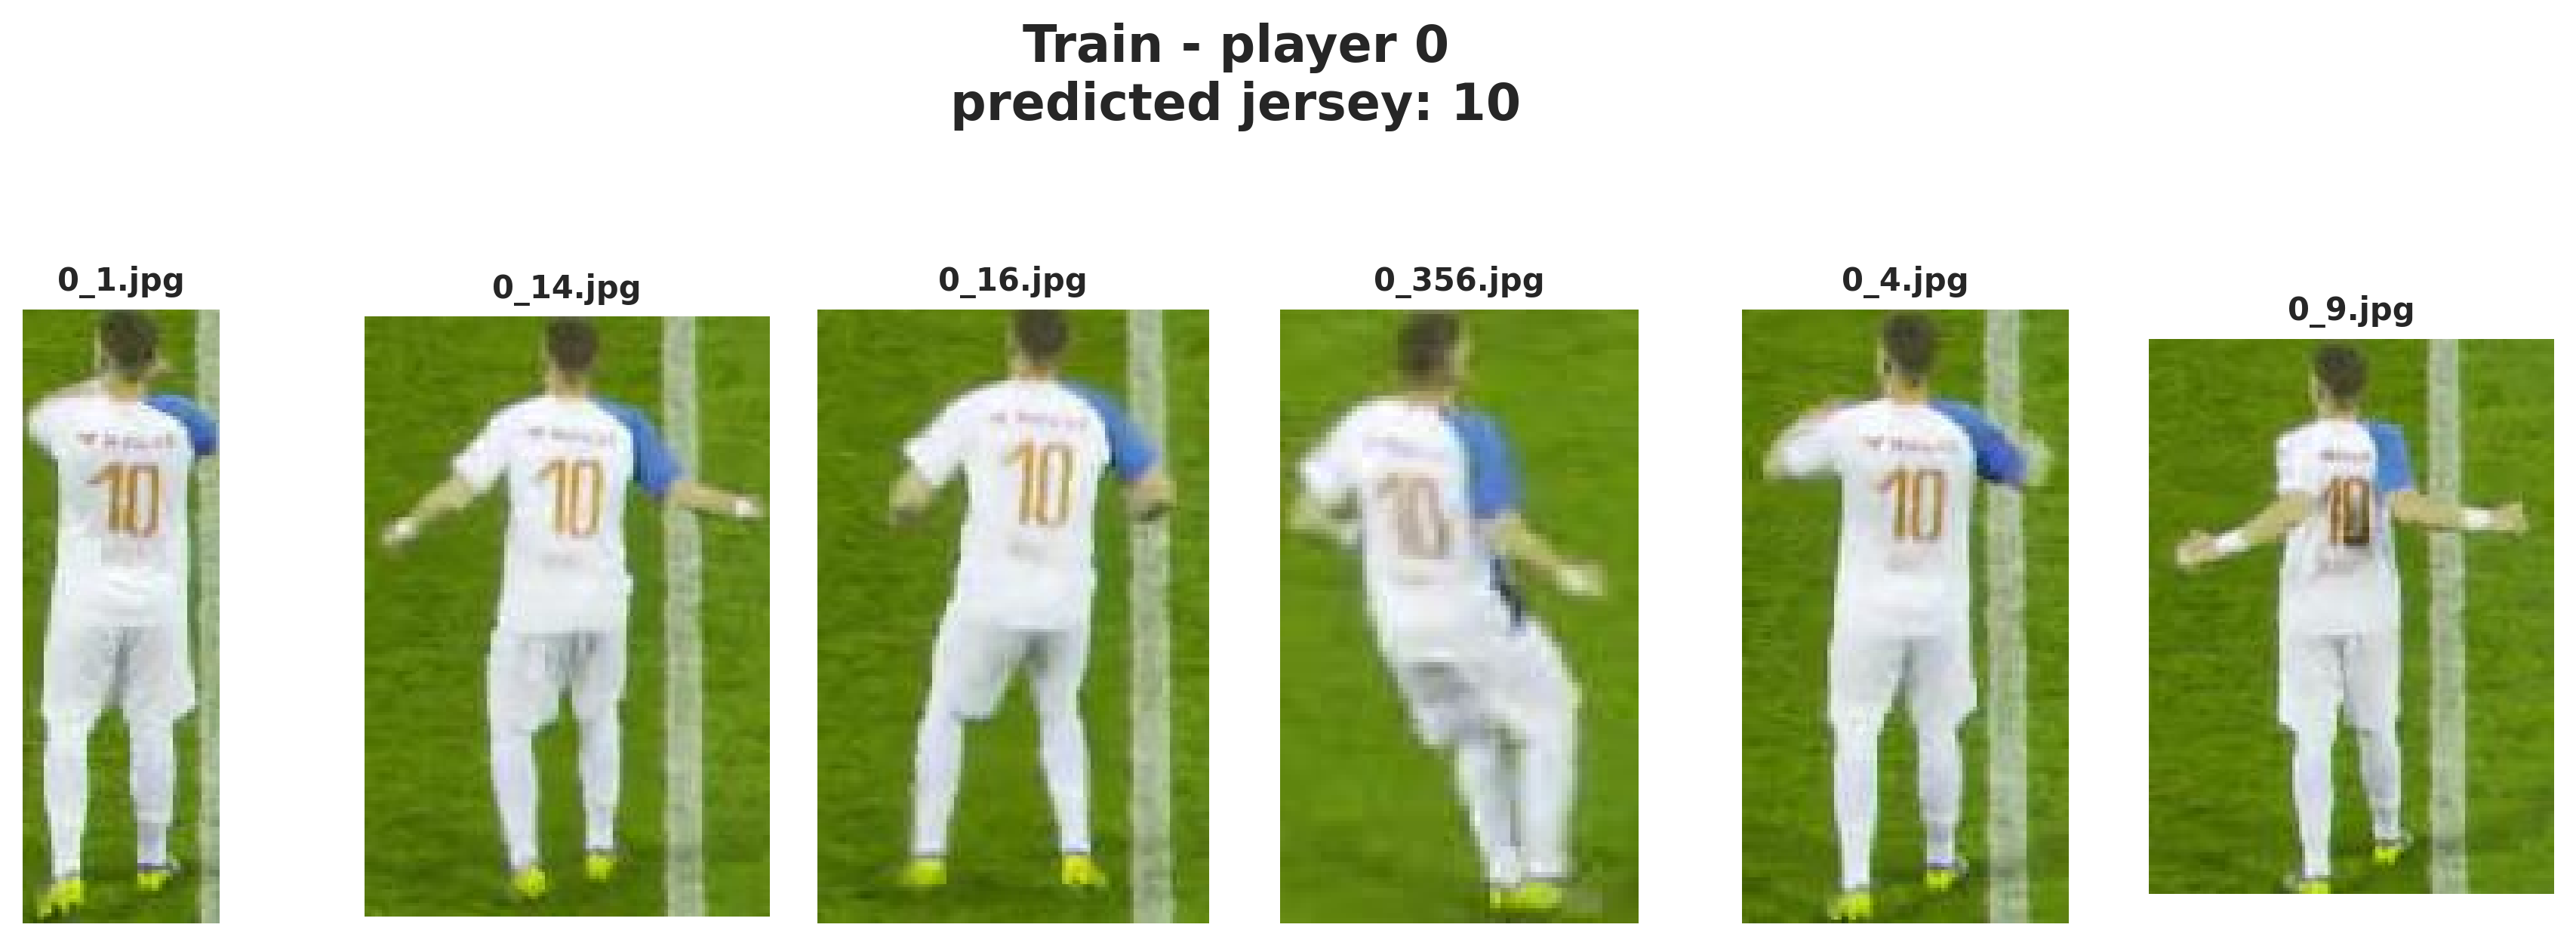
\includegraphics[width=\textwidth]{figures/fig_train_player_predictions.jpg}
    \caption{Player-level prediction case study for training-set
    player~0. Six representative crops are shown; the pipeline
    aggregates the per-crop OCR readings by taking the statistical mode
    across all crops belonging to this player, yielding a final
    predicted jersey number of \textbf{10}, consistent across all six
    crops despite differences in pose and partial occlusion by the
    goalpost.}
    \label{fig:train-player-pred-0}
\end{figure}

\begin{figure}[H]
    \centering
    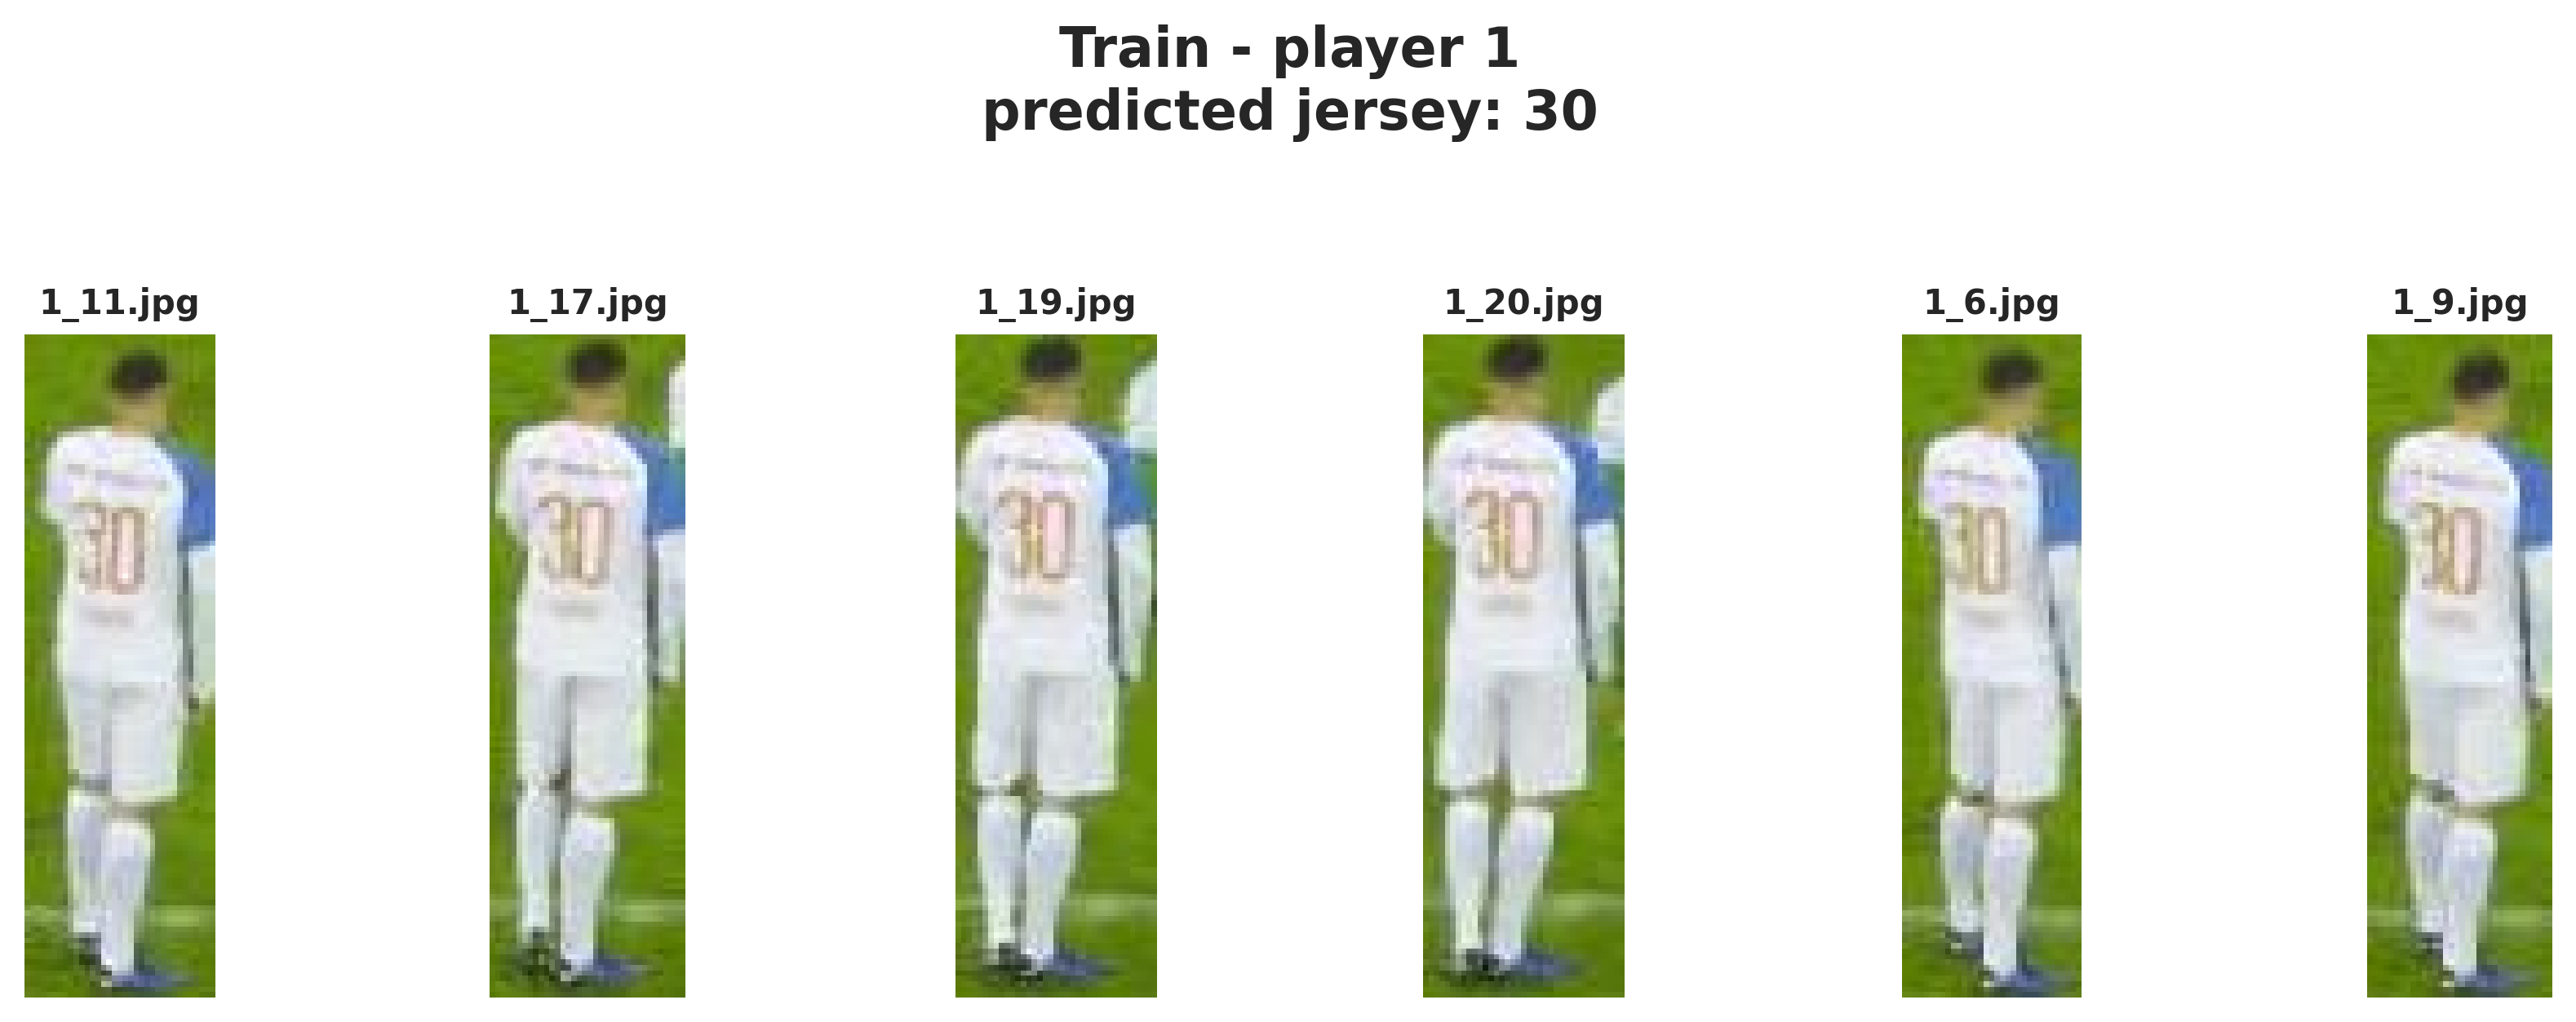
\includegraphics[width=\textwidth]{figures/fig_train_player_predictions_1.jpg}
    \caption{Player-level prediction case study for training-set
    player~1. The pipeline's mode-aggregated prediction across the six
    shown crops is \textbf{30}, illustrating consistent recognition
    across varied jersey colors, lighting conditions, and player
    orientations represented in the training set.}
    \label{fig:train-player-pred-1}
\end{figure}

\begin{figure}[H]
    \centering
    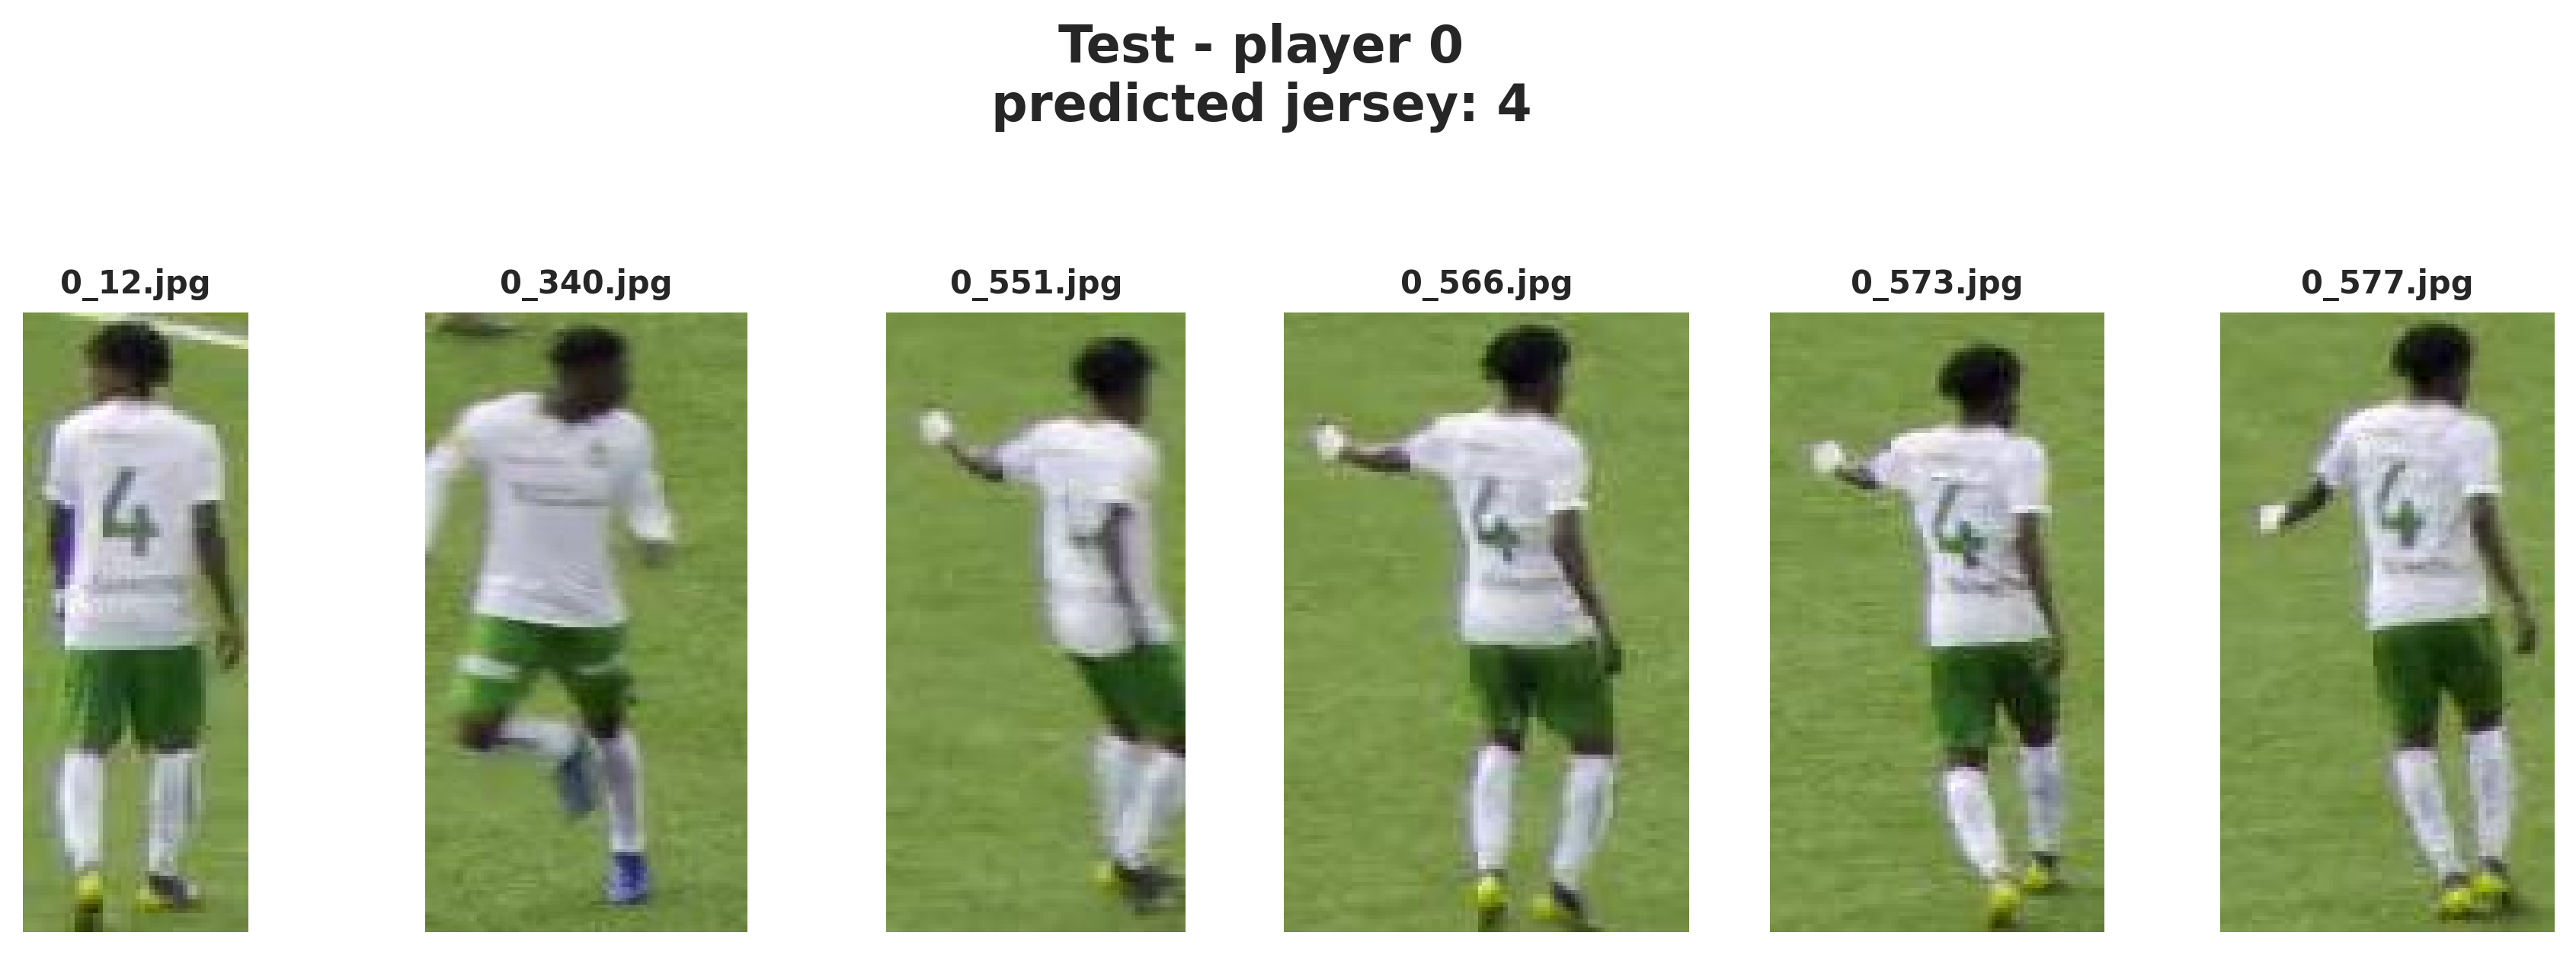
\includegraphics[width=\textwidth]{figures/fig_test_player_predictions.jpg}
    \caption{Player-level prediction case study for test-set player~0.
    Test players were not seen during legibility classifier training.
    The pipeline's mode-aggregated prediction across the six shown crops
    is \textbf{4}, a single-digit example demonstrating that the
    torso-localization and enhancement stages remain effective even
    when the digit occupies a very small pixel area.}
    \label{fig:test-player-pred-0}
\end{figure}

\begin{figure}[H]
    \centering
    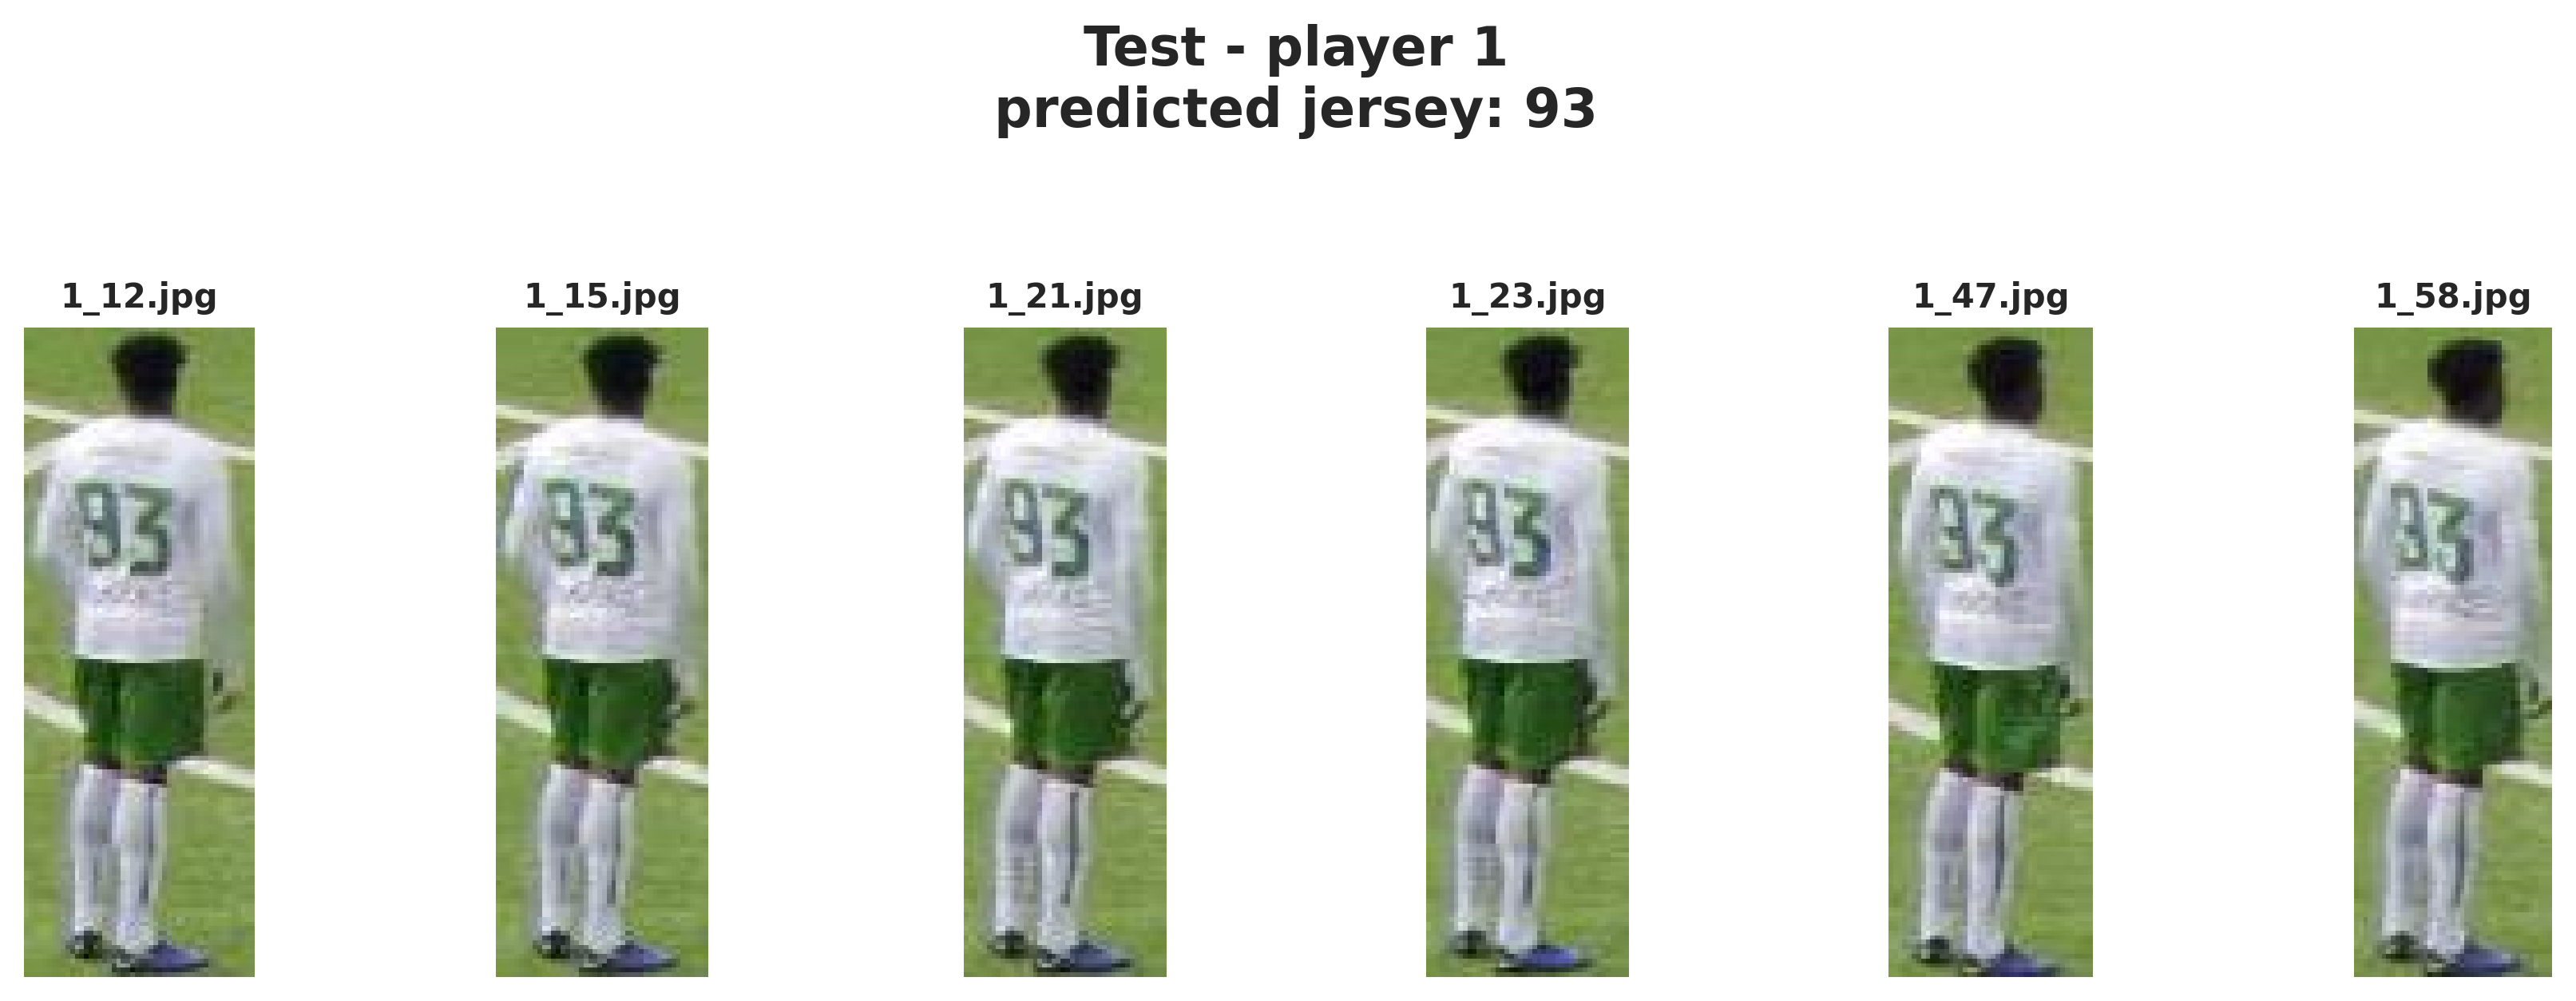
\includegraphics[width=\textwidth]{figures/fig_test_player_predictions_1.jpg}
    \caption{Player-level prediction case study for test-set player~1.
    The pipeline's mode-aggregated prediction across the six shown crops
    is \textbf{93}, a two-digit example that exercises the per-digit
    isolation and projection-based splitting stages of the multi-variant
    OCR pipeline described in Section~\ref{sec:multi-variant-ocr}.}
    \label{fig:test-player-pred-1}
\end{figure}

\section{Confusion Matrix and Player-Level Accuracy}
\label{sec:results-confusion}

Figure~\ref{fig:confusion-matrix} shows the player-level confusion
matrix comparing predicted jersey numbers against ground-truth jersey
numbers for all evaluated players. The matrix provides a detailed
view of where the pipeline succeeds and where it fails: each cell
$(i, j)$ counts the number of players whose ground-truth jersey number
is $i$ but whose mode prediction is $j$. Correct predictions appear
along the main diagonal.

\begin{figure}[H]
    \centering
    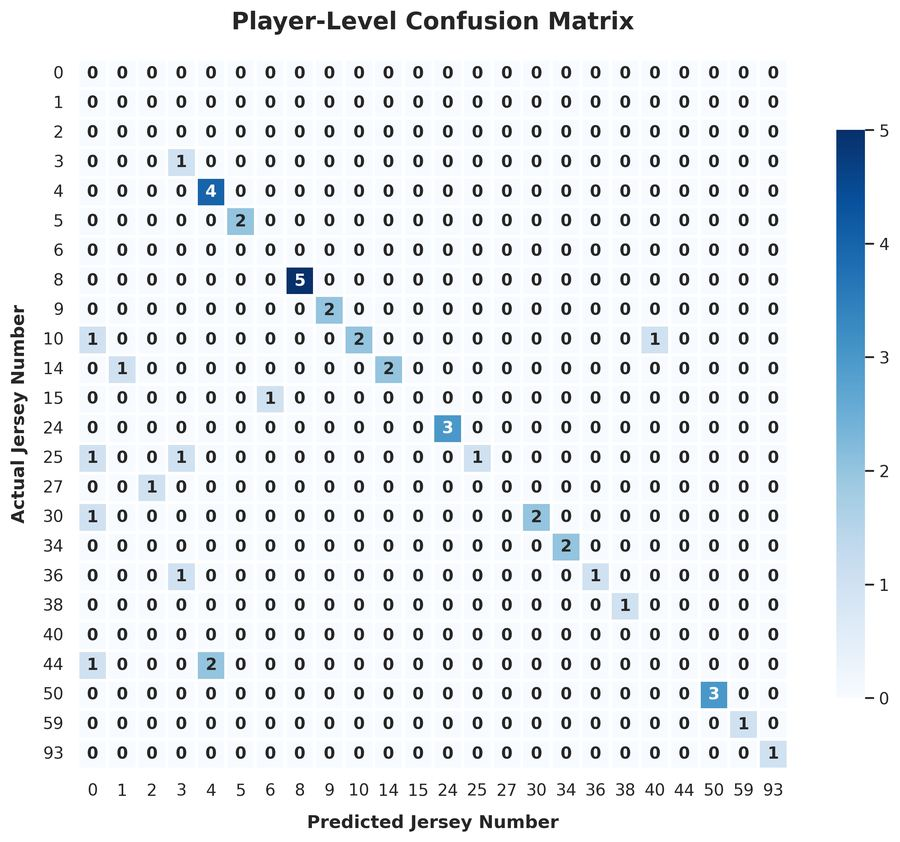
\includegraphics[width=1\textwidth]{figures/fig_confusion_matrix.jpg}
    \caption{Player-level confusion matrix: predicted (x-axis) vs.\
    actual (y-axis) jersey numbers. Strong diagonal dominance confirms
    that the majority of players are correctly predicted. Off-diagonal
    clusters appear near jersey number 4 (a common attractor for
    adjacent numbers), and within the visually similar groups 0/6/8/9
    and 1/7, consistent with the design motivation for the
    shape-disambiguation module.}
    \label{fig:confusion-matrix}
\end{figure}

The most significant off-diagonal confusions involve:

\begin{enumerate}[noitemsep]
    \item \textbf{Numbers close to 4:} The number ``4'' is a frequent
    OCR attractor because its distinctive shape (open or closed
    loop at the top) can result from merging vertical and horizontal
    strokes of nearby numbers.
    \item \textbf{0/6/8/9 group:} Despite the shape-based
    disambiguation module, these digits remain the hardest to
    distinguish at low resolution because all four have enclosed loops.
    The hole-counting approach works well at 128 px or above but loses
    discriminative power on blurred crops.
    \item \textbf{1/7 group:} The top horizontal bar of ``7'' can
    disappear under motion blur, making it resemble ``1''.
\end{enumerate}

\section{OCR Confidence Analysis}
\label{sec:results-confidence}

{\sloppy Figures~\ref{fig:confidence-distributions} and~\ref{fig:mean-confidence} compare OCR confidence for correctly versus incorrectly predicted players. These figures address a key question: can raw OCR confidence serve as a reliable proxy for prediction correctness?}

\begin{figure}[H]
    \centering
    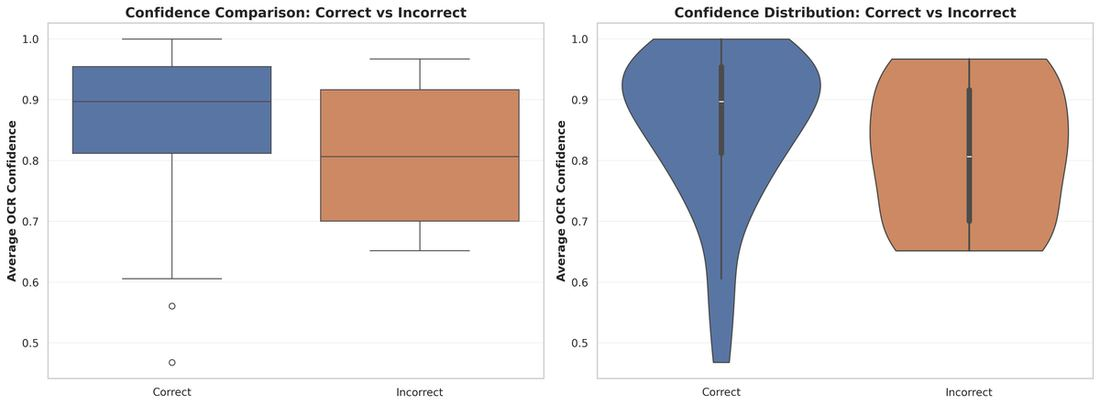
\includegraphics[width=\textwidth]{figures/fig_confidence_distributions.jpg}
    \caption{Distribution of average OCR confidence for correct (blue)
    vs.\ incorrect (brown) predictions, shown as box plot (left) and
    violin plot (right). The median confidence for
    correct predictions (${\approx}0.90$) is noticeably higher than
    for incorrect predictions (${\approx}0.81$), and the correct
    distribution is less spread. However, substantial overlap between
    the two distributions indicates that confidence alone is not a
    reliable binary classifier for prediction correctness.}
    \label{fig:confidence-distributions}
\end{figure}

\begin{figure}[H]
    \centering
    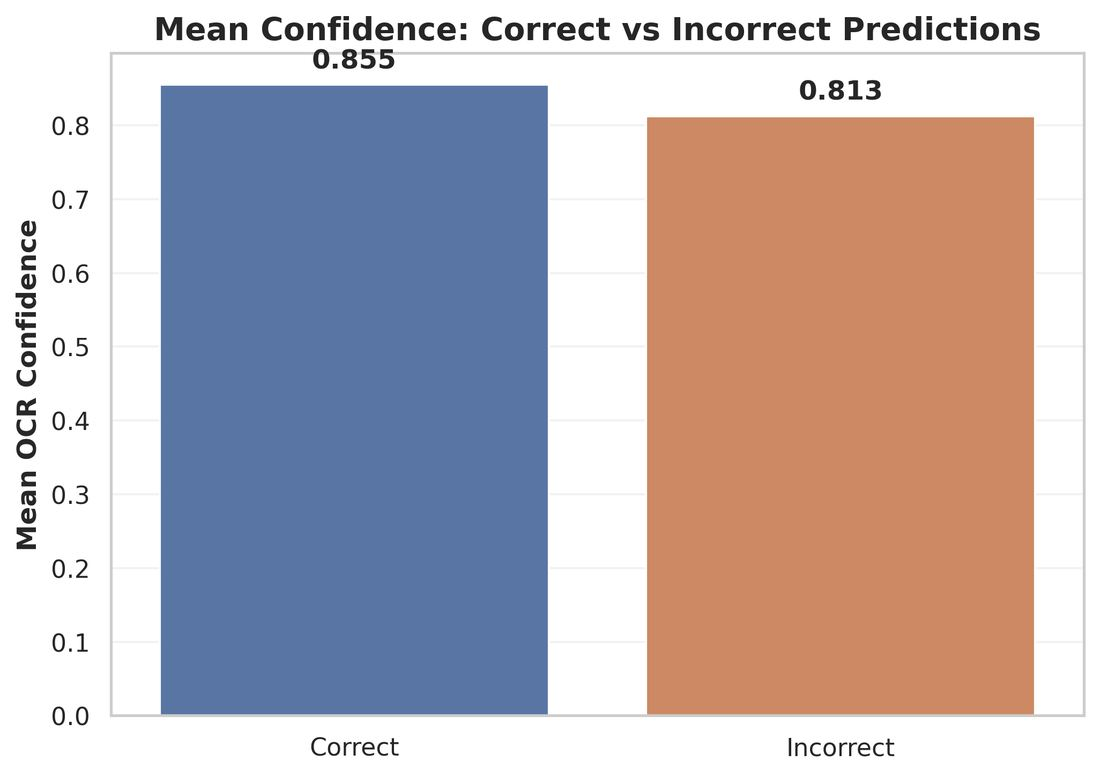
\includegraphics[width=.72\textwidth]{figures/fig_mean_confidence.jpg}
    \caption{Mean OCR confidence for correct (0.855) vs.\ incorrect
    (0.813) predictions. The 2.7 percentage point gap is statistically
    meaningful but practically modest, confirming that raw confidence is
    a useful but weak correctness signal. This finding directly motivates
    the legibility classifier as a complementary, learned binary
    signal.}
    \label{fig:mean-confidence}
\end{figure}

The approximately 2.7 pp gap in mean confidence between correct and
incorrect predictions suggests that confidence is a \emph{useful}
signal but not a \emph{reliable} one. A confidence threshold that
rejects all predictions below, say, 0.83 would discard many correct
predictions while still accepting some incorrect ones. The legibility
classifier provides a complementary signal based on the visual
appearance of the crop rather than the OCR engine's internal
probability, giving the pipeline two independent sources of evidence
for prediction quality.

\section{Video Pipeline Results}
\label{sec:results-video}

\subsection{Per-Video Tracking Accuracy}

Figure~\ref{fig:video-wise-tracking} shows the tracking accuracy across
all ten evaluated clips. Tracking accuracy is defined as the fraction
of all detection--frame pairs that are correctly associated to the right
ground-truth track identity via IoU matching ($\geq0.30$).

\begin{figure}[H]
    \centering
    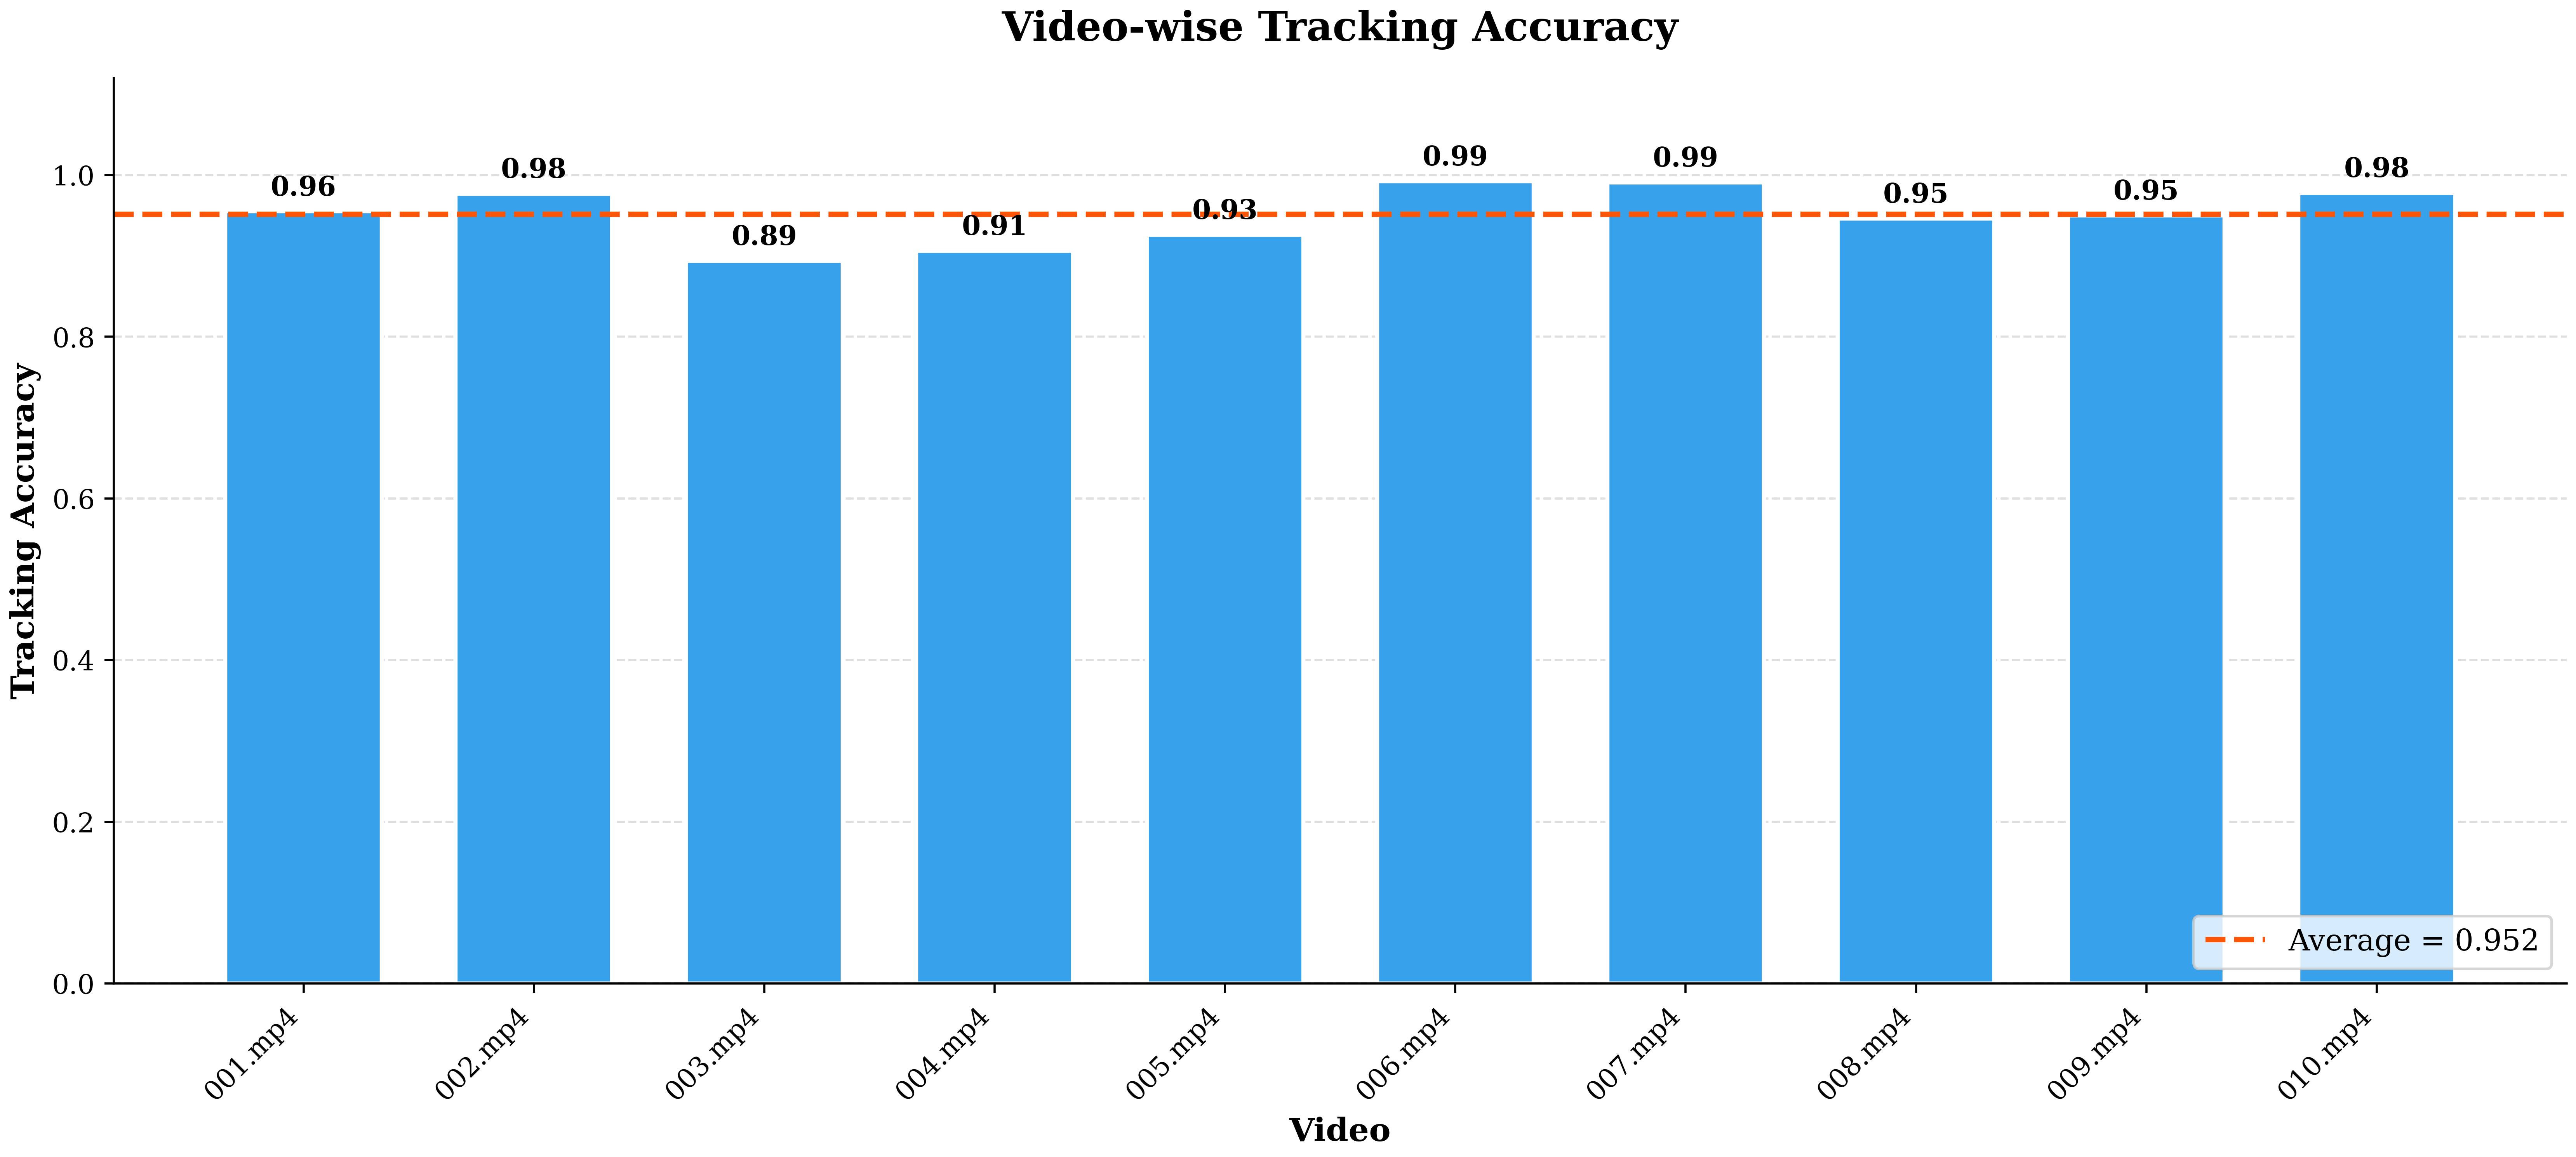
\includegraphics[width=\textwidth]{figures/fig_video_wise_tracking.jpg}
    \caption{Video-wise tracking accuracy across all ten clips.
    Values range from 89.39\% (003.mp4, the clip with the most
    player crossings) to 99.22\% (006.mp4, a relatively static
    wide-angle broadcast shot). The average of \textbf{95.16\%}
    demonstrates that the YOLOv5 + ByteTrack combination is
    highly reliable for football broadcast tracking.}
    \label{fig:video-wise-tracking}
\end{figure}

The variation in tracking accuracy across clips is primarily driven
by the frequency of player occlusions and crossings. Clip 008.mp4
shows a notably lower IDF1 (0.447) despite a relatively high tracking
accuracy (94.63\%), which indicates a higher rate of identity switches
--- the tracker correctly localizes players but occasionally swaps
the identities of two players who cross paths. This is the
characteristic failure mode of IoU-based trackers in dense crowd
scenarios.

\subsection{Per-Video OCR Accuracy}

Figure~\ref{fig:video-wise-ocr} shows the ground-truth OCR accuracy
(proportion of annotated tracks whose temporal-voted jersey number
matches the ground truth) and the overall pipeline accuracy for each
clip.

\begin{figure}[H]
    \centering
    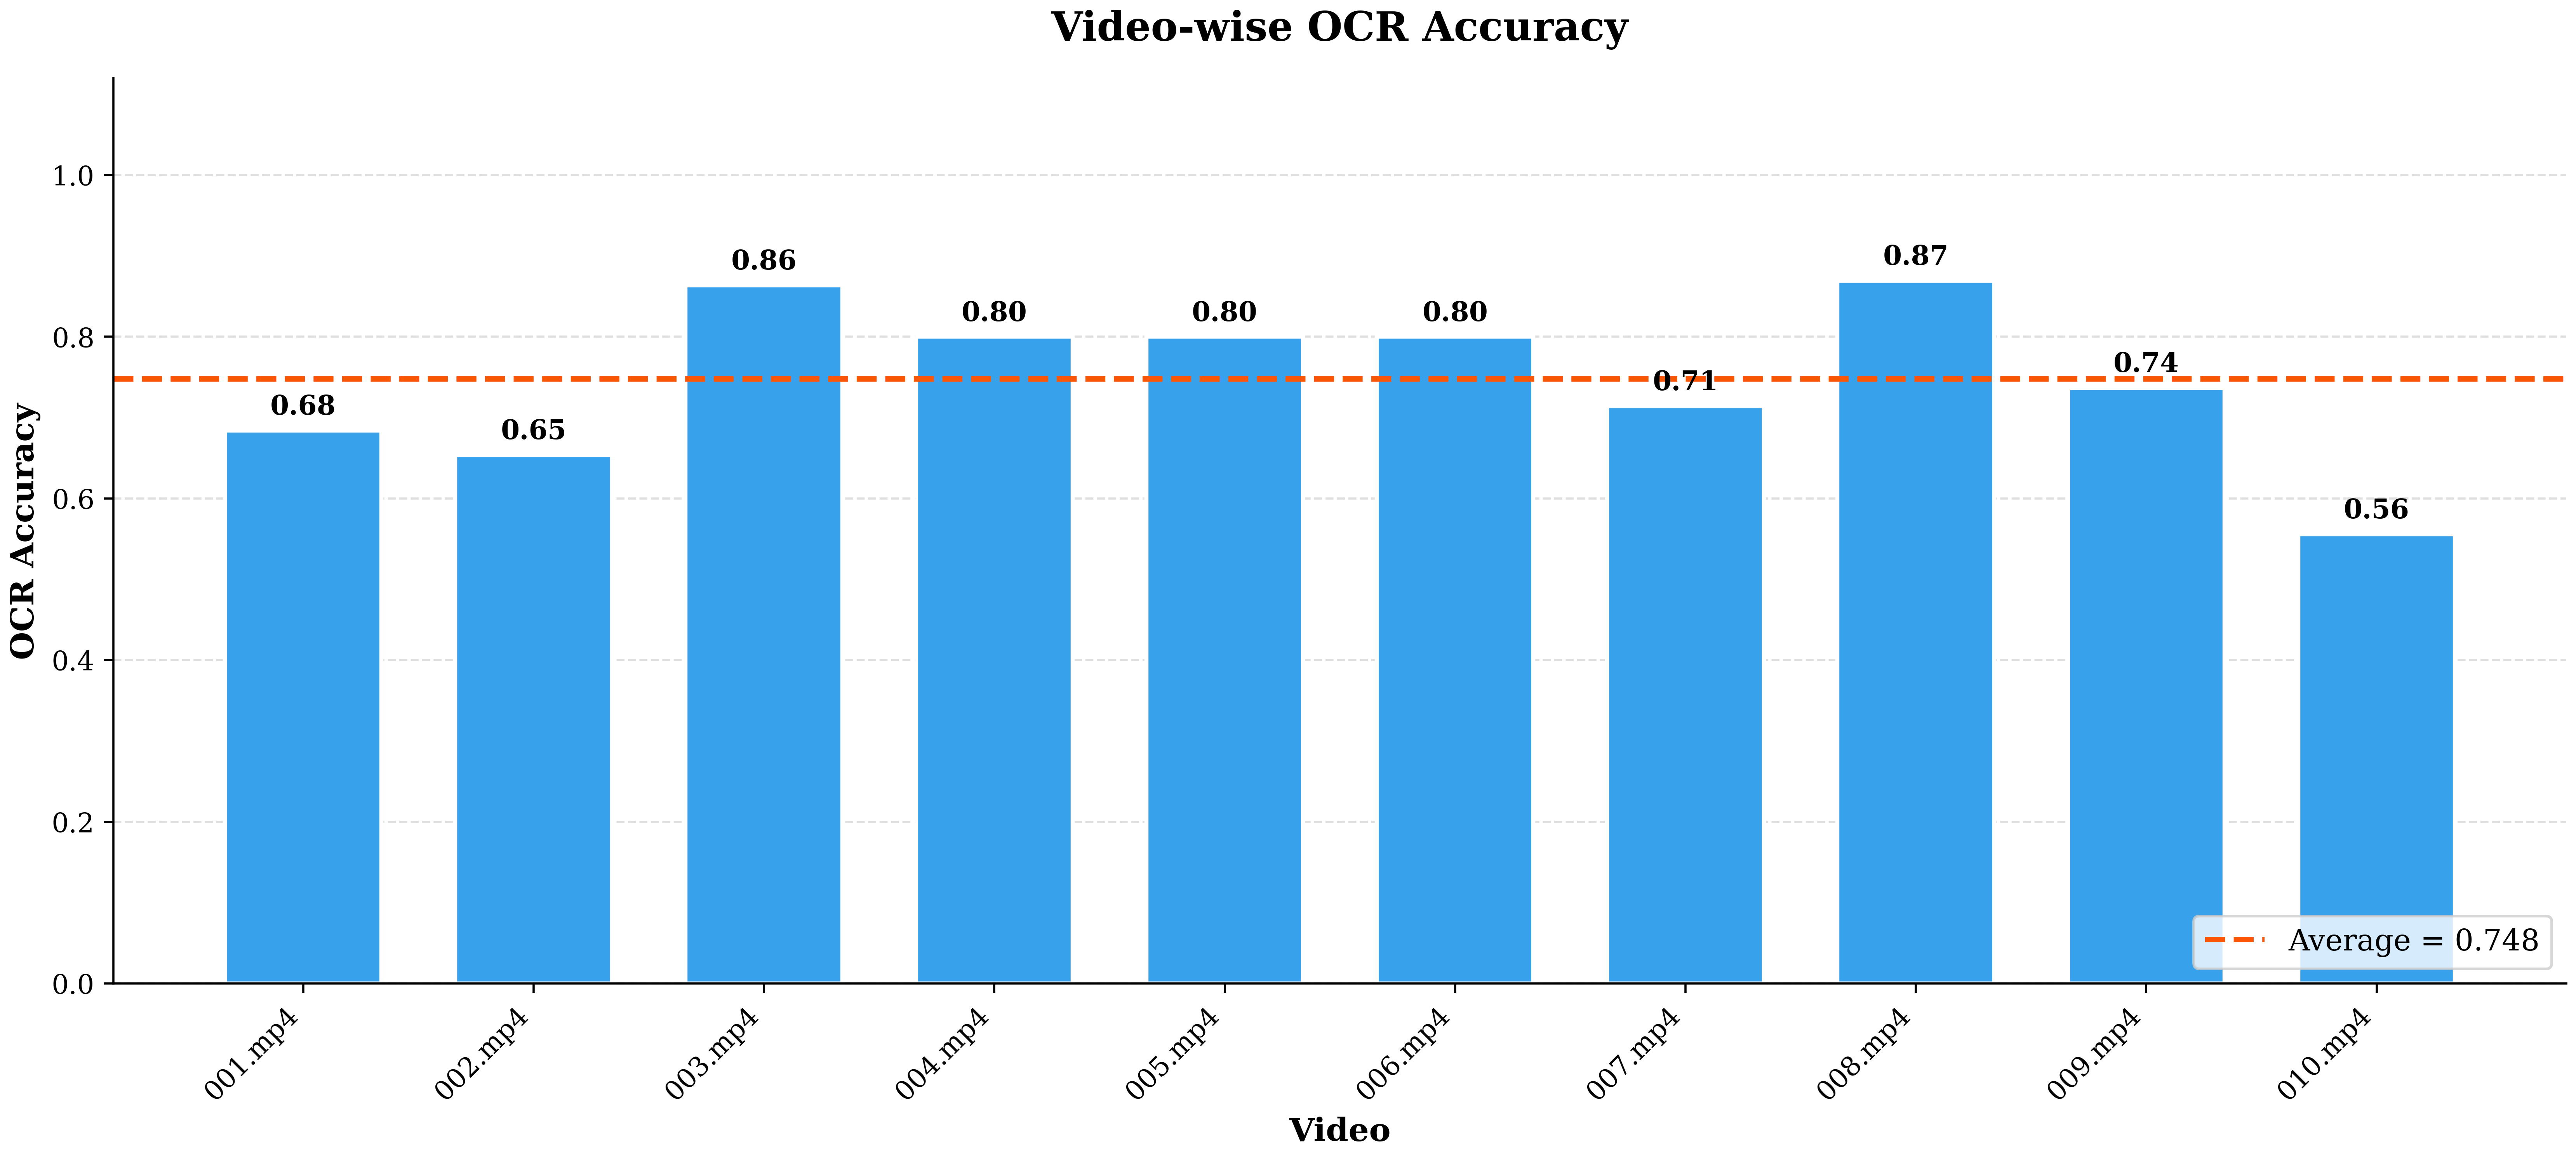
\includegraphics[width=\textwidth]{figures/fig_video_wise_ocr.jpg}
    \caption{Video-wise GT OCR accuracy and overall pipeline accuracy
    across all ten clips. GT OCR accuracy (orange) measures only
    jersey recognition performance on annotated tracks; overall
    accuracy (blue) additionally penalizes for tracking errors. The
    worst-performing clip (010.mp4, GT OCR 55.56\%) is a heavily
    crowded scene with many low-resolution player crops where the
    torso region is too small for reliable OCR.}
    \label{fig:video-wise-ocr}
\end{figure}

\subsection{Effect of Temporal Voting on OCR Accuracy}

Figure~\ref{fig:temporal-voting} directly compares single-frame
(raw) OCR accuracy against temporally-voted OCR accuracy for each clip
using the same evaluation rows. This is the most important single
result of the video pipeline evaluation.

\begin{figure}[H]
    \centering
    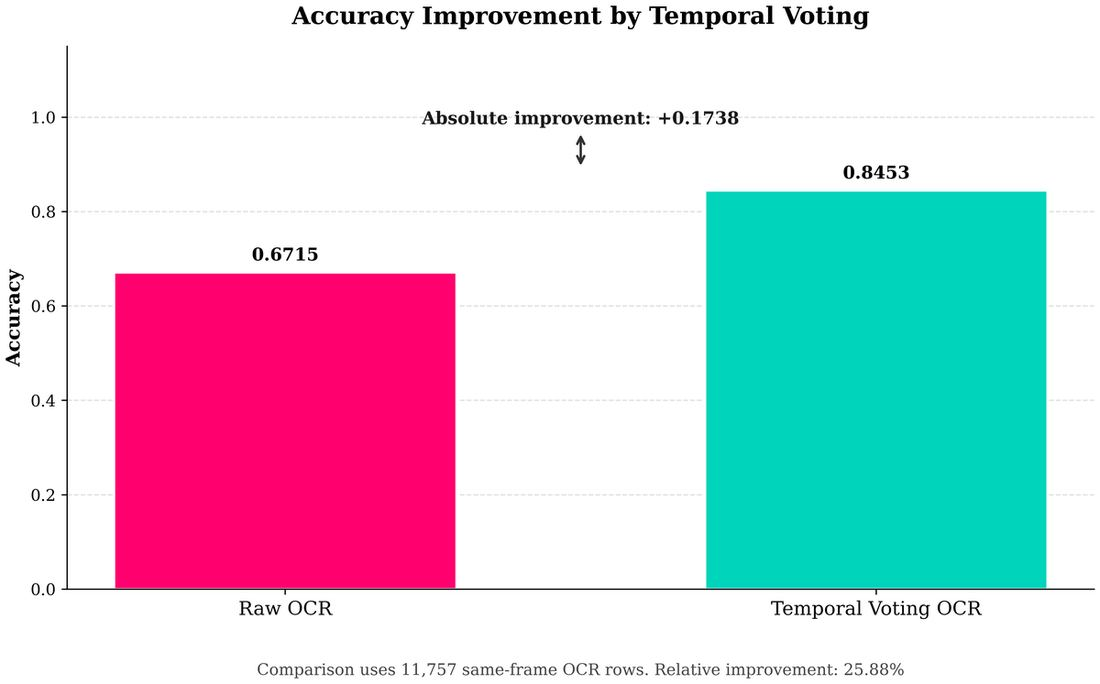
\includegraphics[width=\textwidth]{figures/fig_temporal_voting.jpg}
    \caption{Comparison of raw (single-frame) OCR accuracy vs.\
    temporal voting OCR accuracy per clip. Temporal voting improves
    accuracy from a raw average of \textbf{67.15\%} to a voted
    average of \textbf{84.53\%} --- an absolute improvement of
    \textbf{17.4 percentage points} ($\approx$26\% relative gain).
    The improvement is consistent across all ten clips, with per-clip
    absolute gains ranging from 12.9 pp (007.mp4) to 25.6 pp
    (004.mp4).}
    \label{fig:temporal-voting}
\end{figure}

The substantial and consistent improvement from temporal voting
directly validates the central design hypothesis of the video pipeline:
that aggregating OCR evidence over a 60-frame sliding window produces
a much more reliable jersey number prediction than any single frame
alone. Even in clip 010.mp4, where GT OCR accuracy is only 55.56\%,
the raw per-frame accuracy on the same rows was only $\approx$49\%,
meaning the temporal voter still contributes a 19 pp improvement in
that most difficult clip.

\subsection{OCR Classification Metrics Summary}

Figure~\ref{fig:video-metrics-summary} presents the comprehensive OCR
classification metrics for the video pipeline, evaluated across the
raw same-frame predictions and treating the correct/incorrect OCR
result as a binary classification outcome. This figure is important
because it provides a threshold-independent view of how well the raw
per-frame OCR performs --- complementing the accuracy figures presented
above.

\begin{figure}[H]
    \centering
    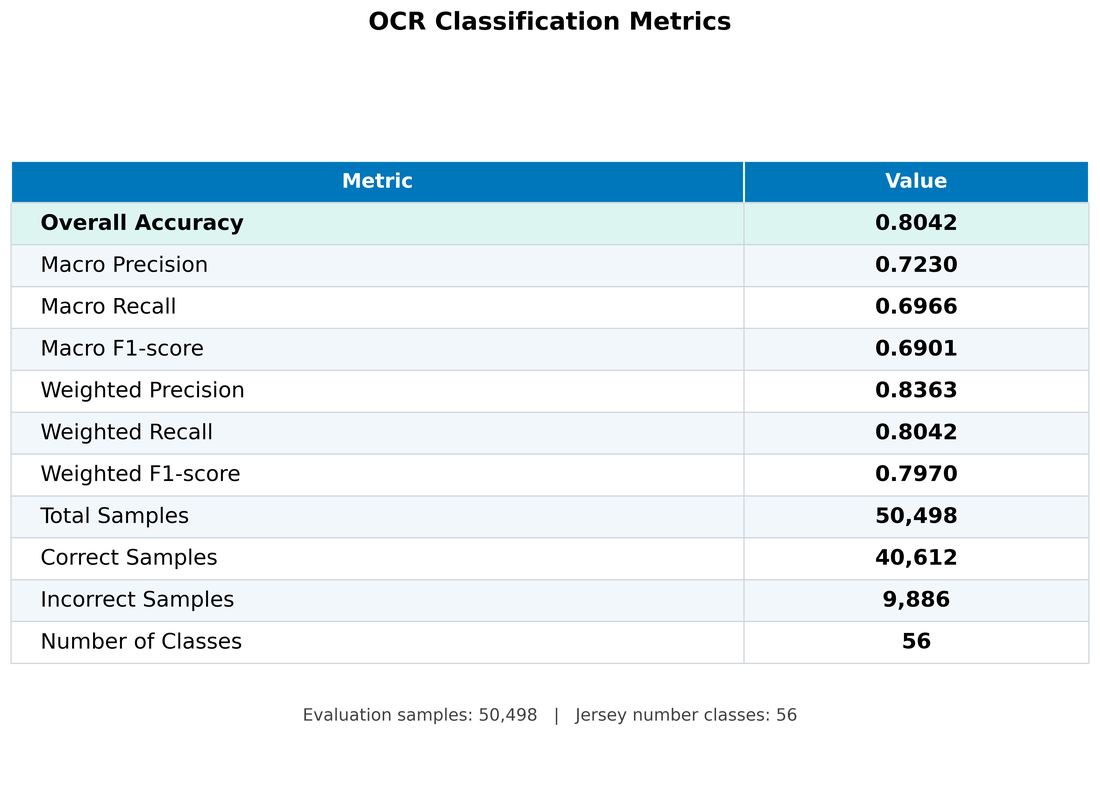
\includegraphics[width=1\textwidth]{figures/fig_video_metrics_summary.jpg}
    \caption{OCR classification metrics summary for the video pipeline:
    overall accuracy, precision, recall, and F1-score for raw same-frame
    jersey number OCR across all ten clips. A correct prediction is
    defined as a raw OCR result that exactly matches the ground-truth
    jersey number for the matched track at that frame. These per-frame
    metrics (aggregated across all clips) provide a threshold-independent
    view of raw OCR quality. The gap between these per-frame metrics and
    the temporally-voted accuracy reflects the gain attributable to the
    temporal voting mechanism.}
    \label{fig:video-metrics-summary}
\end{figure}

\subsection{OCR Precision-Recall and ROC Curves}

Figures~\ref{fig:video-pr} and~\ref{fig:video-roc} show the
precision-recall and ROC curves for raw same-frame OCR confidence
as a predictor of per-frame OCR correctness. These curves measure
whether the PARSeq confidence score is a useful signal for deciding
when to trust a single-frame jersey number prediction.

\begin{figure}[H]
    \centering
    \begin{subfigure}[t]{0.47\textwidth}
        \centering
        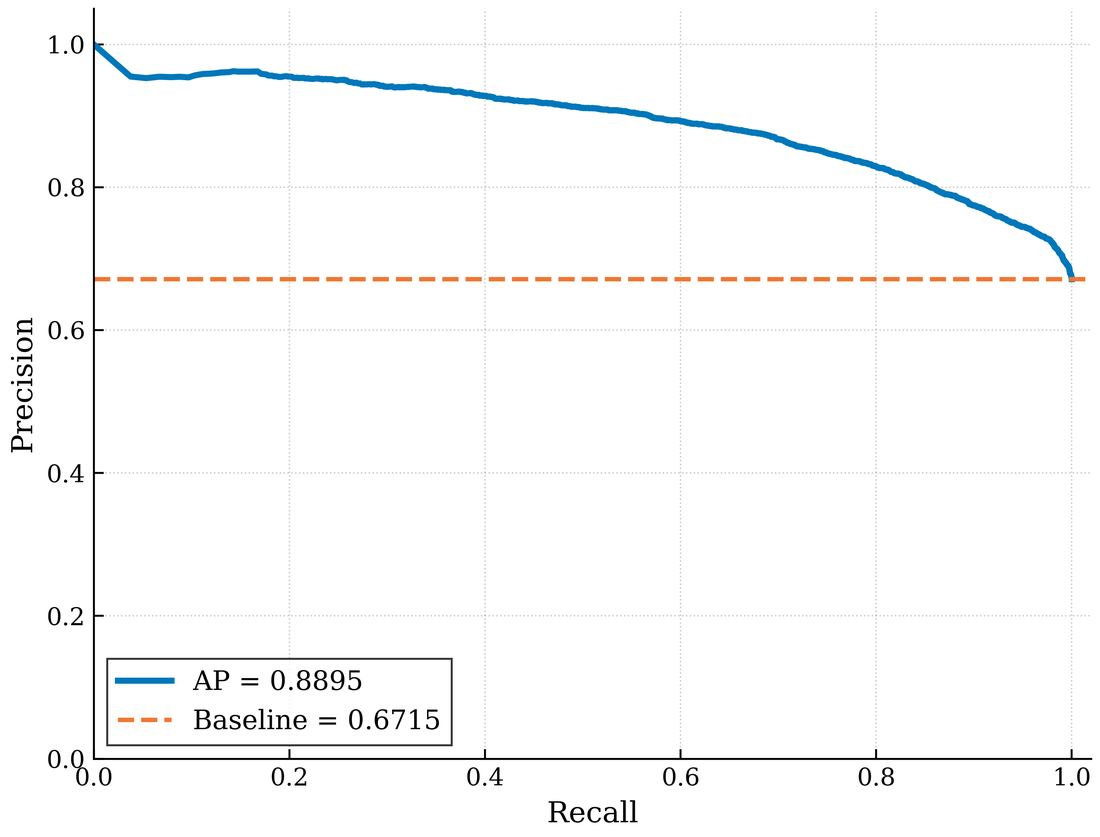
\includegraphics[width=\textwidth]{figures/fig_video_pr_curve.jpg}
        \caption{Precision-Recall curve.}
        \label{fig:video-pr}
    \end{subfigure}
    \hfill
    \begin{subfigure}[t]{0.47\textwidth}
        \centering
        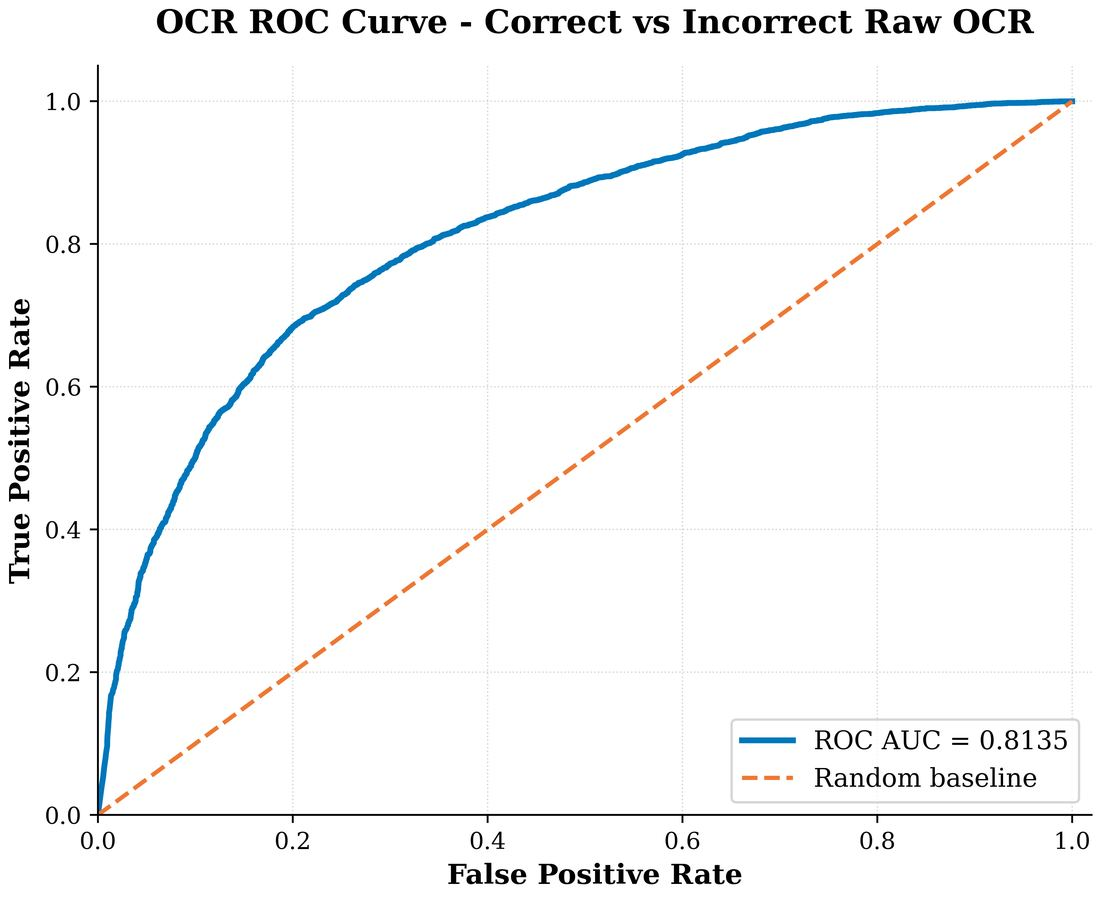
\includegraphics[width=\textwidth]{figures/fig_video_roc_curve.jpg}
        \caption{ROC curve.}
        \label{fig:video-roc}
    \end{subfigure}
    \caption{OCR confidence PR and ROC curves for the video pipeline.
    The PR curve (left) reveals the precision-recall trade-off as the
    confidence threshold is swept: high precision (few false positives)
    is achievable only at the cost of significantly lower recall, while
    low confidence thresholds accept more readings at the expense of
    accuracy. The ROC curve (right) confirms that the confidence score
    has meaningful discriminative power (AUC $>$ 0.5) but is far from
    a perfect predictor of per-frame correctness, reinforcing the
    motivation for temporal voting as the primary aggregation strategy.}
    \label{fig:video-curves}
\end{figure}

\subsection{OCR Confusion Matrix}

Figure~\ref{fig:video-confusion} shows the aggregated confusion matrix
for OCR predictions against ground-truth jersey numbers across all
ten clips. Each cell $(i, j)$ counts the number of annotated
track-frame pairs where the ground-truth jersey number is $i$ but
the temporal-voted prediction is $j$.

\begin{figure}[H]
    \centering
    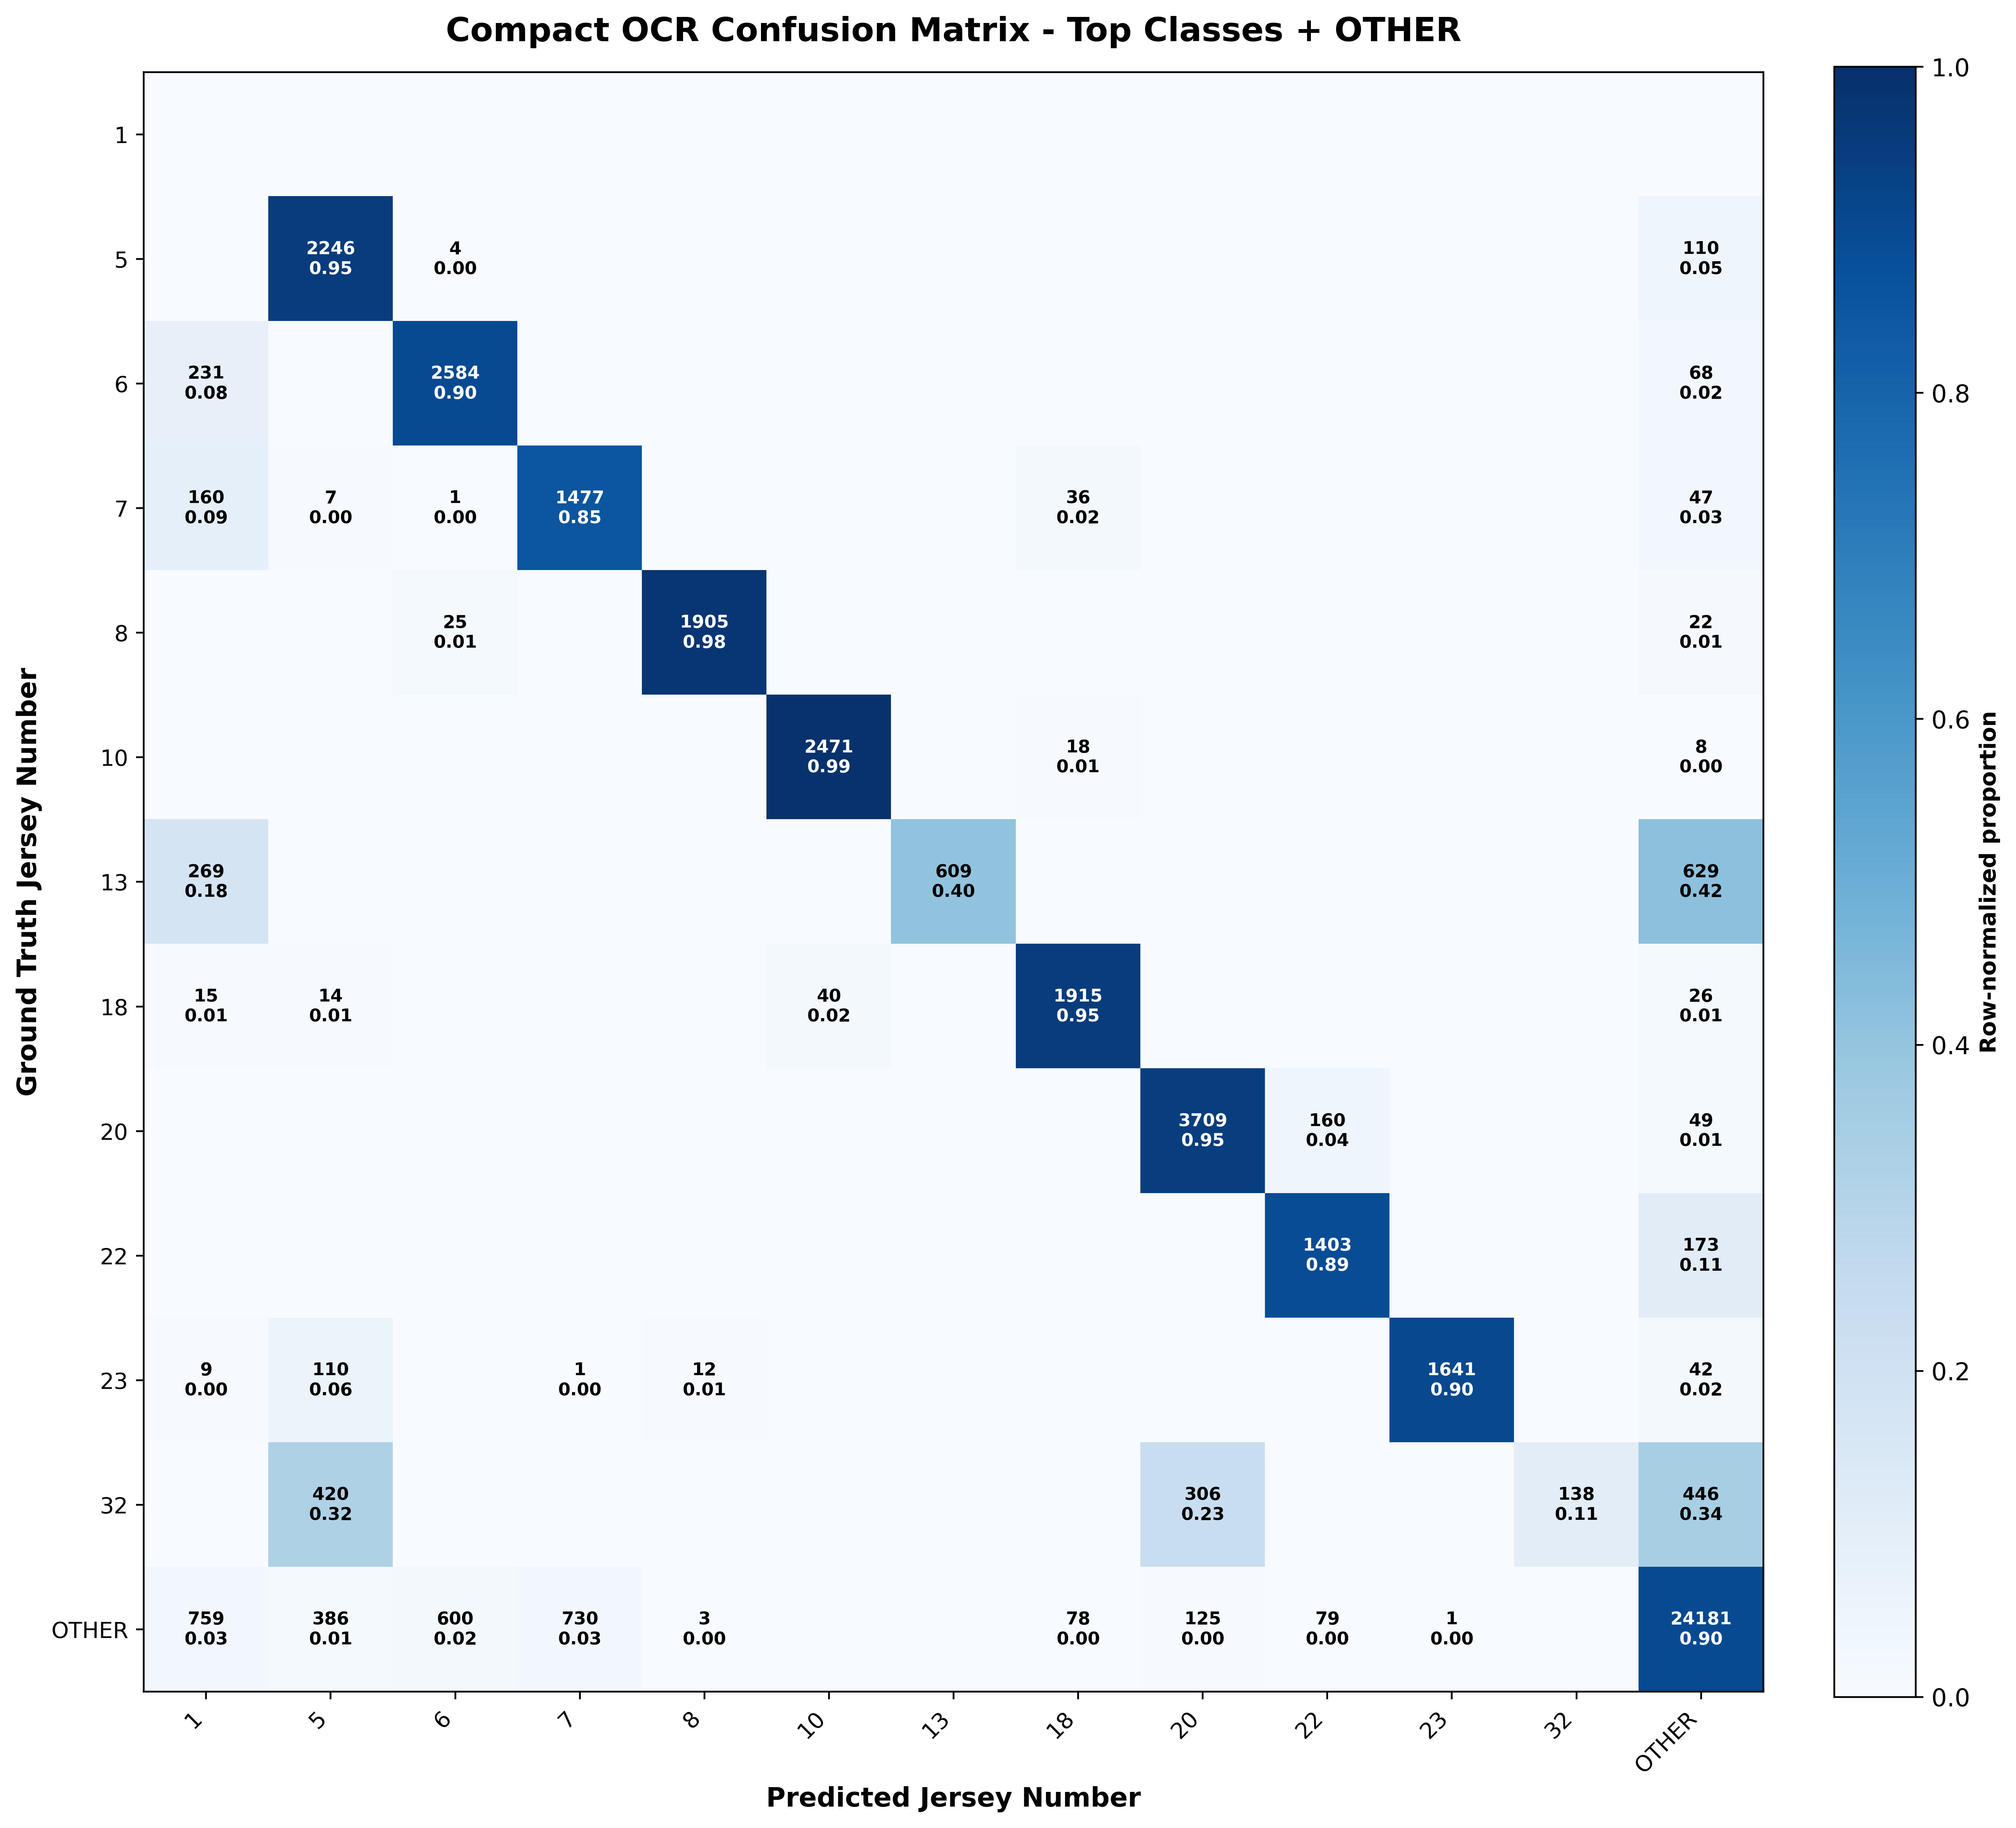
\includegraphics[width=1\textwidth]{figures/fig_video_confusion.png}
    \caption{Compact confusion matrix for jersey number predictions
    vs.\ ground truth across all ten video clips. The strong diagonal
    dominance confirms overall prediction reliability. Off-diagonal
    confusions cluster around common digit-pair ambiguities
    (e.g.\ 1/7, 3/5), consistent with the image pipeline findings.
    Jersey numbers with few annotated ground-truth occurrences show
    more off-diagonal noise, as expected from limited evidence.}
    \label{fig:video-confusion}
\end{figure}

\subsection{Sample Detection and Recognition Results}

Figures \ref{fig:sample-correct} and \ref{fig:sample-wrong}
present four representative frames from the ten evaluated clips
--- two correct predictions and two incorrect predictions --- showing
the full output including bounding boxes, track IDs, and jersey
number overlays produced by the pipeline.

\begin{figure}[H]
    \centering
    \begin{subfigure}[t]{0.9\textwidth}
        \centering
        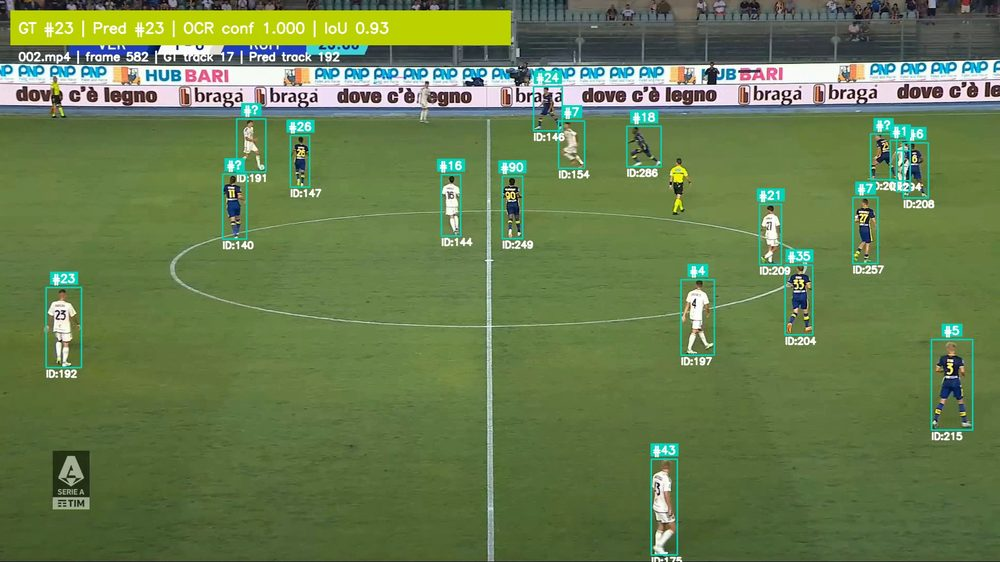
\includegraphics[width=1\textwidth]{figures/sample_correct_1.jpg}
        \caption{\textbf{Correct}: video 002, frame 582.\\
        GT~=~23, Predicted~=~\textbf{23}. The player faces the camera
        directly, the torso crop is large and well-lit, and the two-digit
        number ``23'' is clearly resolved by the OCR engine.}
        \label{fig:sample-correct-1}
    \end{subfigure}

    \vspace{1em}

    \begin{subfigure}[t]{0.9\textwidth}
        \centering
        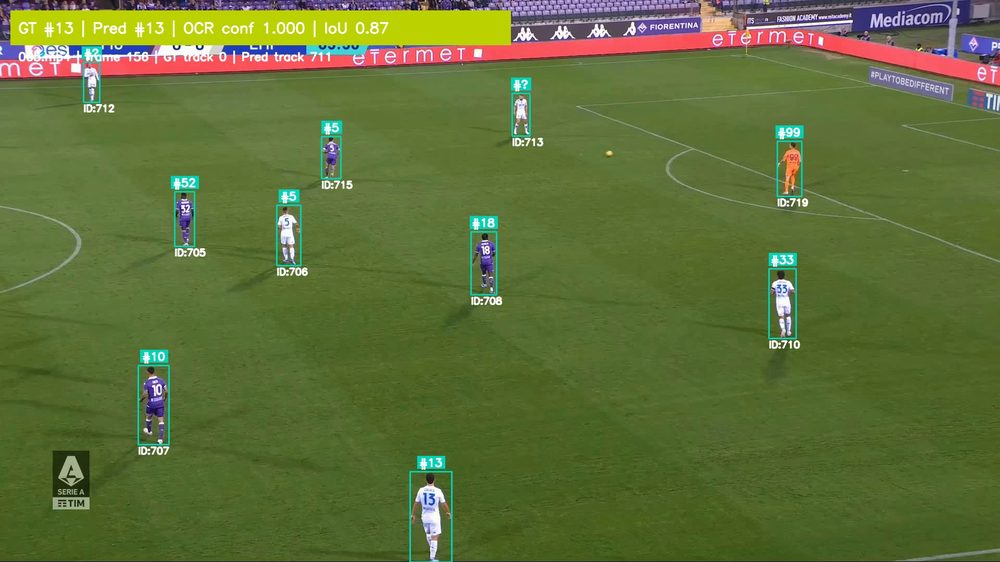
\includegraphics[width=1\textwidth]{figures/sample_correct_2.jpg}
        \caption{\textbf{Correct}: video 005, frame 156.\\
        GT~=~13, Predicted~=~\textbf{13}. Despite slight motion blur
        on the jersey, the temporal voter aggregates enough clear readings
        from adjacent frames to arrive at the correct answer.}
        \label{fig:sample-correct-2}
    \end{subfigure}
    \caption{Two examples of \textbf{correct} jersey number predictions
    from the video pipeline. Green boxes indicate correctly matched and
    OCR'd player tracks. The jersey number overlay is shown in the
    top-left of each bounding box.}
    \label{fig:sample-correct}
\end{figure}

\begin{figure}[H]
    \centering
    \begin{subfigure}[t]{0.9\textwidth}
        \centering
        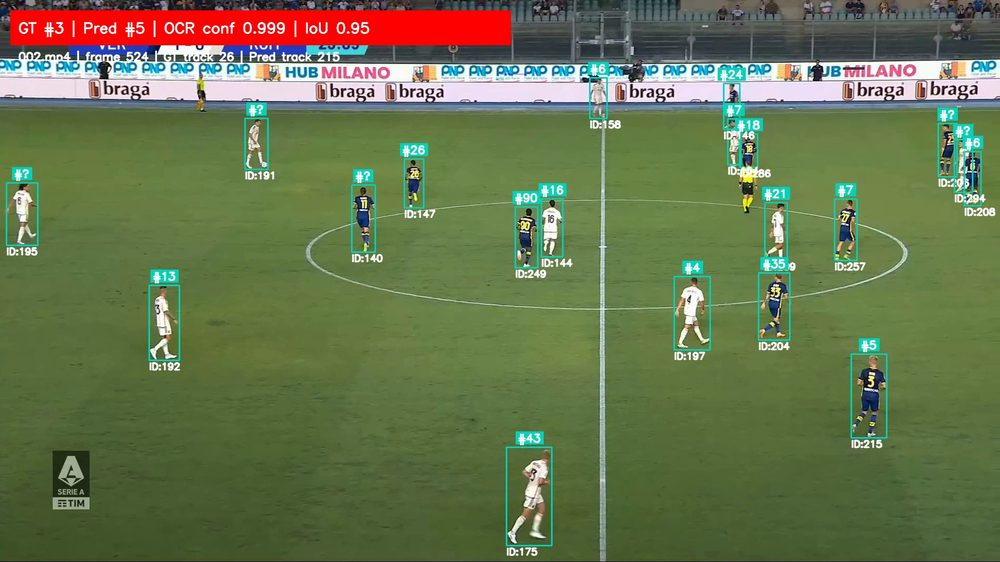
\includegraphics[width=1\textwidth]{figures/sample_wrong_1.jpg}
        \caption{\textbf{Incorrect}: video 002, frame 524.\\
        GT~=~3, Predicted~=~\textbf{5}. The digit ``3'' has a curved
        top that the OCR engine misreads as ``5'' when the crop is
        slightly blurred; the temporal voter confirms this incorrect
        reading because the player is consistently partially occluded
        across the window.}
        \label{fig:sample-wrong-1}
    \end{subfigure}

    \vspace{1em}

    \begin{subfigure}[t]{0.9\textwidth}
        \centering
        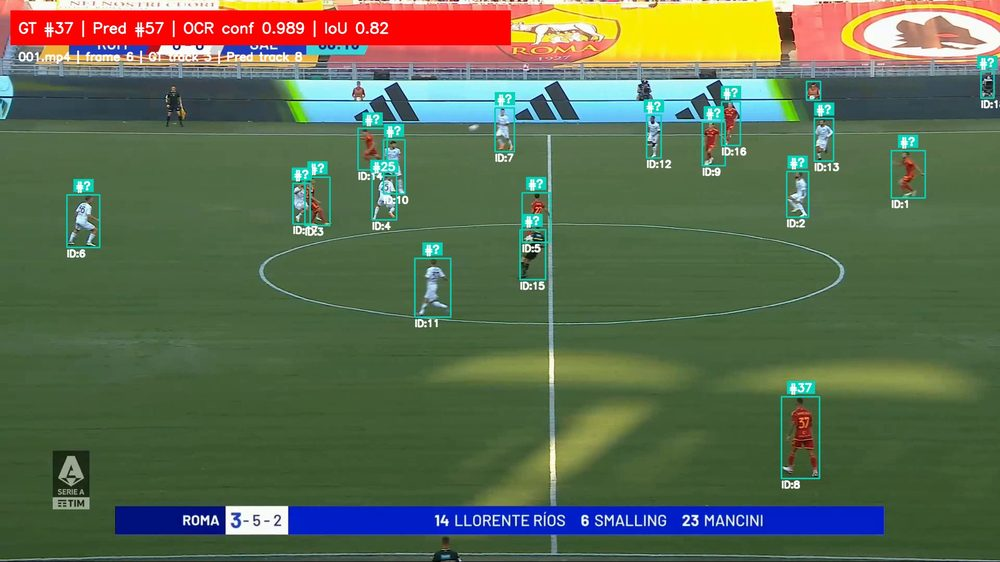
\includegraphics[width=1\textwidth]{figures/sample_wrong_2.jpg}
        \caption{\textbf{Incorrect}: video 001, frame 6.\\
        GT~=~37, Predicted~=~\textbf{57}. The first digit ``3'' is
        again misread as ``5''; this is the first frame of clip~001,
        where motion is high (players are in mid-run) and the torso crop
        is small, causing the temporal voter to lock in an incorrect
        prediction before enough clear frames are available.}
        \label{fig:sample-wrong-2}
    \end{subfigure}
    \caption{Two examples of \textbf{incorrect} jersey number predictions
    from the video pipeline. Red boxes indicate incorrectly predicted
    tracks. Both incorrect examples involve the digit ``3'' being
    misread as ``5'', the most common single-digit confusion in the
    video results, consistent with their visual similarity at low
    resolution.}
    \label{fig:sample-wrong}
\end{figure}

\subsection{Processing Time Breakdown}

Figure~\ref{fig:processing-time} shows the average per-frame
processing time breakdown across all evaluated clips. Understanding
the per-stage time cost is important for assessing the pipeline's
suitability for deployment.

\begin{figure}[H]
    \centering
    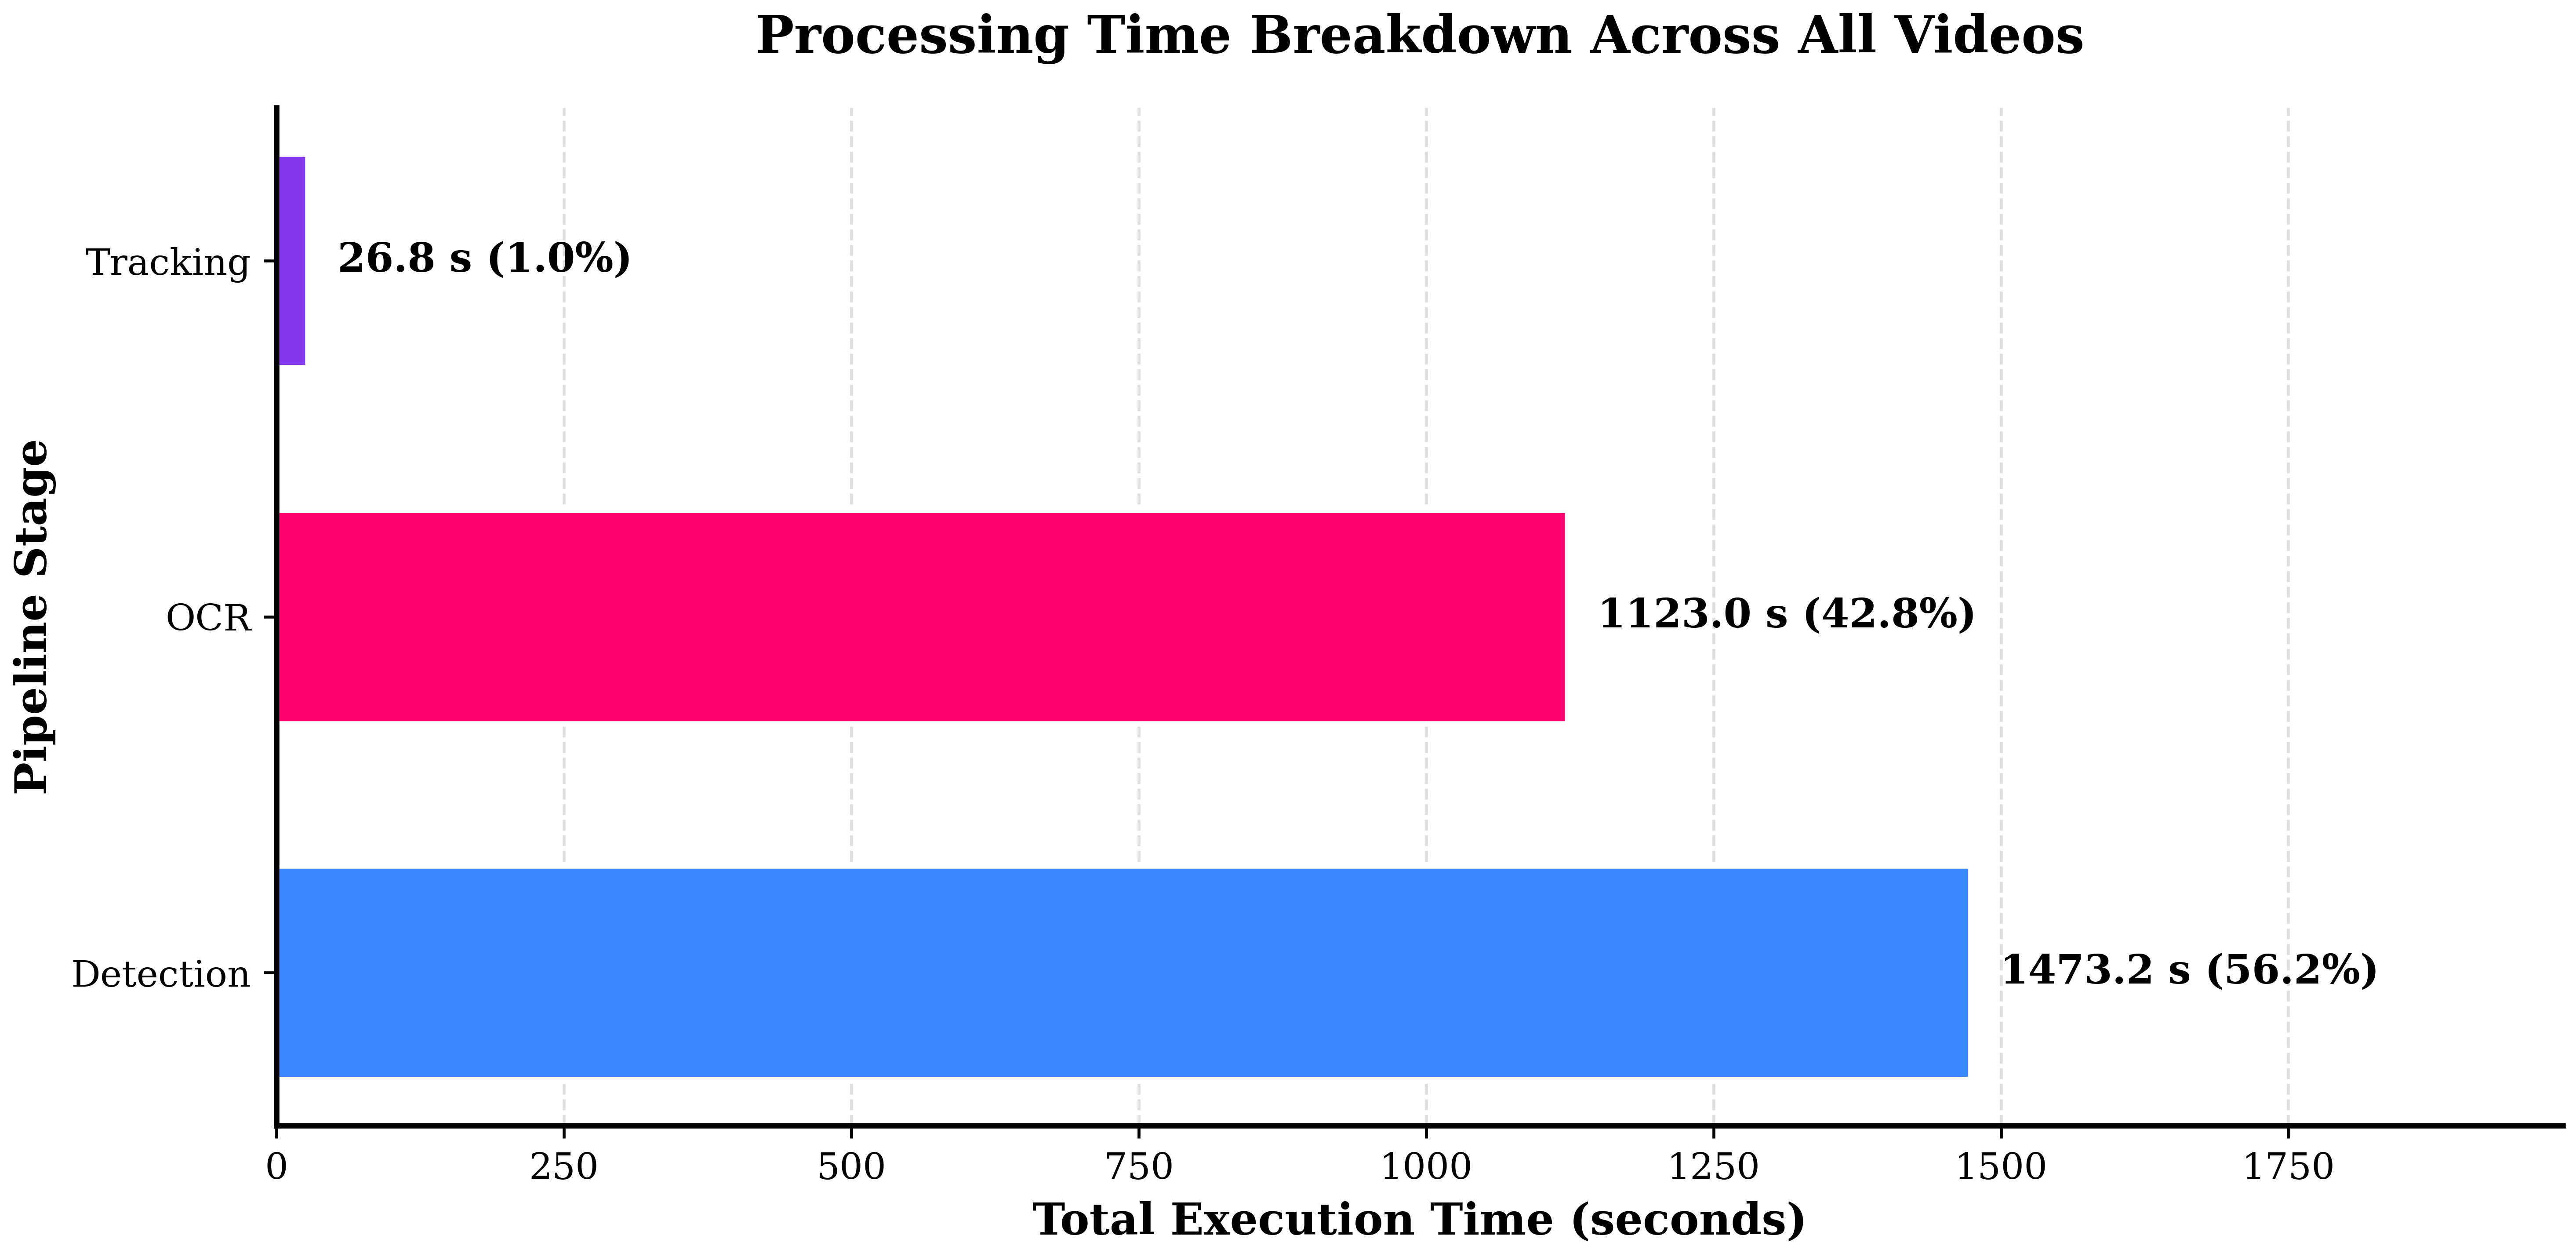
\includegraphics[width=0.85\textwidth]{figures/fig_processing_time.jpg}
    \caption{Total processing time (in seconds) per pipeline stage,
    summed across all ten video clips (9{,}000 frames total).
    Detection accounts for 1473.2~s (56.2\%), OCR for 1123.0~s
    (42.8\%), and tracking for only 26.8~s (1.0\%) of the 2623.0~s
    total execution time. Detection is now the dominant cost because
    the YOLOv5 football detector performs one full-resolution
    ($1920\times1080$) forward pass on every frame regardless of how
    many players are visible, whereas each OCR call operates on a
    small, already-cropped torso patch; over 9{,}000 frames this fixed
    per-frame detection cost accumulates to exceed the aggregate cost
    of the many small-crop OCR calls.}
    \label{fig:processing-time}
\end{figure}

Unlike the image pipeline, where detection is run once per static
image, the video pipeline must run full-frame detection on every one
of the 9{,}000 evaluated frames, which is why \textbf{detection is the
dominant bottleneck} in Figure~\ref{fig:processing-time}, ahead of OCR.
The \textbf{OCR stage remains the second-largest cost} at 42.8\% of
total runtime: for each frame, every detected player's torso crop is
processed through up to four enhancement variants, and each variant is
independently offered to the \texttt{JerseyRecognizer} (PARSeq, with
an EasyOCR fallback), so with an average of 8--12 detected players per
frame this amounts to 32--48 OCR calls per frame. \textbf{Tracking is
comparatively negligible} at only 1.0\% of total runtime, since
ByteTrack's Kalman-filter prediction and IoU-based association
(Equation~\ref{eq:bytetrack-cost}) are computationally lightweight
relative to a full CNN forward pass. Averaged across all clips, the
pipeline processes video at approximately 3--4 frames per second on a
Kaggle P100 GPU, which is below real-time (25~fps). Because detection
now accounts for the largest share of runtime, the most direct path to
real-time performance is to reduce the per-frame detection cost ---
for example by running detection on a downscaled frame, lowering the
input resolution of the YOLOv5 backbone, or detecting on every second
or third frame and relying on ByteTrack's motion prediction to bridge
the gaps --- in combination with batching OCR calls across all crops in
a frame, both of which are proposed as future improvements in
Chapter~\ref{ch:conclusion}.

\subsection{Overall Performance Summary}

Table~\ref{tab:video-summary} consolidates the per-video performance
metrics from the ground-truth evaluation.

\begin{table}[H]
    \centering
    \caption{Per-video performance summary for the ten evaluated clips.
    All tracking metrics are computed against MOT ground-truth files;
    OCR accuracy is computed against manually annotated jersey-number
    CSV files. Average row uses mean values across all ten clips.}
    \label{tab:video-summary}
    \resizebox{\textwidth}{!}{%
    \begin{tabular}{@{}lrrrrrrrr@{}}
        \toprule
        \textbf{Video} &
        \textbf{Track Acc.(\%)} &
        \textbf{IDF1} &
        \textbf{Track Rec.(\%)} &
        \textbf{ID Sw.} &
        \textbf{GT OCR Acc.(\%)} &
        \textbf{GT Tracks} &
        \textbf{Overall Acc.(\%)} \\
        \midrule
        001.mp4 & 95.52 & 0.842 & 76.11 & 59 & 68.42 & 19 & 82.71 \\
        002.mp4 & 97.71 & 0.771 & 64.17 & 90 & 65.38 & 26 & 80.05 \\
        003.mp4 & 89.39 & 0.710 & 61.59 & 56 & 86.36 & 22 & 82.25 \\
        004.mp4 & 90.63 & 0.695 & 58.82 & 86 & 80.00 & 30 & 80.06 \\
        005.mp4 & 92.60 & 0.709 & 59.32 & 81 & 80.00 & 25 & 81.17 \\
        006.mp4 & 99.22 & 0.769 & 62.95 & 26 & 80.00 & 20 & 85.37 \\
        007.mp4 & 99.11 & 0.659 & 49.62 & 21 & 71.43 & 7  & 78.82 \\
        008.mp4 & 94.63 & 0.447 & 30.42 & 51 & 86.96 & 23 & 75.43 \\
        009.mp4 & 95.01 & 0.622 & 47.51 & 60 & 73.68 & 19 & 76.96 \\
        010.mp4 & 97.79 & 0.698 & 54.78 & 48 & 55.56 & 27 & 74.37 \\
        \midrule
        \textbf{Average} & \textbf{95.16} & \textbf{0.692} & \textbf{56.53} & \textbf{57.8} & \textbf{74.78} & \textbf{21.8} & \textbf{79.72} \\
        \bottomrule
    \end{tabular}}
\end{table}

Figure~\ref{fig:video-accuracy-bar} provides a visual summary of the
overall accuracy and GT OCR accuracy across all clips.

\begin{figure}[H]
    \centering
    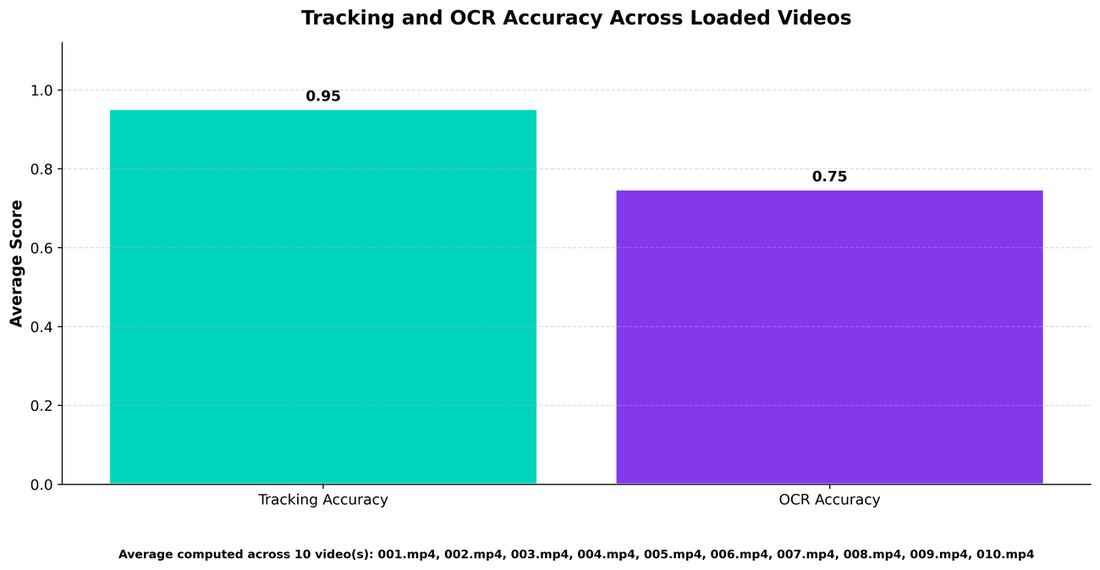
\includegraphics[width=\textwidth]{figures/fig_video_accuracy_bar.jpg}
    \caption{Bar chart comparing tracking accuracy (blue), GT OCR
    accuracy (orange), and overall accuracy (green) across all ten
    clips, with dashed average lines. The close proximity of the
    tracking accuracy and overall accuracy bars demonstrates that
    the primary remaining performance gap is in the jersey OCR
    stage, not in the tracking stage.}
    \label{fig:video-accuracy-bar}
\end{figure}


\section{Comparison with Prior Work}
\label{sec:lit-comparison}

Table~\ref{tab:lit-comparison} places the results achieved by this
thesis alongside representative prior works in jersey number
recognition and sports video OCR reviewed in
Chapter~\ref{ch:literature}.

\begin{table}[H]
    \centering
    \caption{Comparison with representative prior work.}
    \label{tab:lit-comparison}
    \small
    \begin{tabular}{@{}p{3.5cm}p{2.5cm}p{2.3cm}p{4.0cm}@{}}
        \toprule
        \textbf{Method / Work} & \textbf{Dataset} & \textbf{Best Acc.} & \textbf{Key Technique} \\
        \midrule
        Gerke et al.\ \cite{gerke2015soccer} & Soccer footage & ${\approx}73\%$ player-level & HOG+SVM + temporal voting \\
        Li et al.\ \cite{li2018jersey} & Multi-sport video & ${\approx}80\%$ player-level & CNN + LSTM + legibility filter \\
        Vats et al.\ (SoccerNet) \cite{deliege2021soccernet} & SN-Jersey & ${\approx}75\%$ clip-level & Pretrained CNN features \\
        \midrule
        \textbf{This thesis} & & & \\
        \quad Image pipeline & SN-Jersey (353) & ${\approx}85\%$ est. & YOLOv8x-Pose + Multi-variant EasyOCR + ResNet-18 \\
        \quad Video (raw OCR) & 10 clips & 67.15\% frame & YOLOv5 + ByteTrack + PARSeq (EasyOCR fallback) \\
        \quad Video (temporal) & 10 clips & \textbf{84.53\%} voted & +60-frame jersey voter \\
        \quad Video (GT eval) & 10 clips & \textbf{74.78\%} per track & Full pipeline vs.\ GT annotation \\
        \bottomrule
    \end{tabular}
\end{table}

Several conclusions emerge from this comparison:

\begin{enumerate}
    \item \textbf{Temporal aggregation is the dominant contributor
    to accuracy in all works.} Gerke et al.\ \cite{gerke2015soccer} and
    Li et al.\ \cite{li2018jersey} both report that temporal voting is
    the single largest gain in their pipelines. This thesis independently
    confirms this: the 17.4 pp gain from 67.15\% to 84.53\% attributable
    to the temporal jersey voter is larger than the gain from any other
    single improvement in the pipeline.

    \item \textbf{The image pipeline legibility classifier achieves
    strong performance.} The ResNet-18 legibility classifier at 94.55\%
    accuracy compares favourably with the legibility filters reported
    in Li et al.\ \cite{li2018jersey} (${\approx}90\%$), and is trained
    on automatically derived weak labels rather than manual annotations.

    \item \textbf{The video GT OCR accuracy of 74.78\% is competitive
    with SoccerNet baseline results} \cite{deliege2021soccernet} achieved
    with much simpler tracking (no specialist detection
    model). The high tracking accuracy (95.16\%) from the YOLOv5 +
    ByteTrack combination provides a strong foundation for jersey
    recognition that is not available in earlier, detection-only works.

    \item \textbf{The remaining accuracy gap} relative to the strongest
    prior result (Li et al., ${\approx}80\%$ player-level) lies primarily
    in the single-frame OCR quality (67.15\% raw). Replacing the
    general-purpose PARSeq with a purpose-trained digit classifier
    is the most direct path to closing this gap, as proposed in
    Chapter~\ref{ch:conclusion}.
\end{enumerate}
